\documentclass[12pt, a4paper]{article}


\usepackage{setspace}
\usepackage[utf8]{inputenc}
\usepackage{amsmath}
\usepackage{amsfonts}
\usepackage{amssymb}
\usepackage{ngerman}


\usepackage{tabularx}


\parindent 0pt

% Seitenformat festlegen
\usepackage{geometry}
\geometry{a4paper, top=25mm, left=35mm, right=25mm, bottom=20mm, headheight=15mm, headsep=10mm, footskip=12mm}

\usepackage{nameref}
\usepackage{graphicx}
%\usepackage[update,prepend]{epstopdf}
%\usepackage{siunitx}
\usepackage{here}
\usepackage{listings}
\usepackage{color}

\usepackage{pgfplots}
\usepackage{pgfplotstable}

\usepackage{hyperref}

\usepackage{fancyhdr}
\pagestyle{fancy}
\fancyhf{}
\fancyhead[L]{\textit{ {\leftmark}}}
\fancyfoot[C]{\thepage}

\usepackage{acronym}

\parindent 0pt



 

\begin{document}



\definecolor{MMLComment}{rgb} {0.53, 0.54, 0.52}
\definecolor{MMLEmph}   {rgb} {0.58, 0.00, 0.82}
\definecolor{MMLString} {rgb} {0.86, 0.44, 0.00}
\definecolor{MMLKeyword}{rgb} {0.20, 0.39, 0.64}

\lstdefinelanguage{mml}{
    sensitive=false,
    alsoletter={\# \< \>},
    morecomment=[l]{;},
    commentstyle=\color{MMLComment},
    emphstyle=\color{MMLEmph}\textbf,
    emph={
        \#samples,
        \#default,
        \#optimized,
        \#instruments,
        \#pad,
        \#spc,
        \#author,
        \#game,
        \#comment,
        \#title,
        \#length,
        \#path,
        \#halvetempo,
        \#option,
        \#define,
        \#undef,
        \#ifdef,
        \#ifndef,
        \#if,
        \#endif,
        \#error,
        \#amk,
        \#0,
        \#1,
        \#2,
        \#3,
        \#4,
        \#5,
        \#6,
        \#7,
    },
    keywordstyle=\color{MMLKeyword}\textbf,
    morekeywords={
        w180,
        t32,
        \<,
        \>,
    },
}


\newpage

\begin{titlepage}
    \begin{center}
        \vspace*{1cm}
            
        \Huge
        \textbf{Tutorial zum Porten und Schreiben von 16 Bit Songs mit AddMusicK}
            
        \vspace{0.5cm}
        \LARGE

            
        \vspace{1.5cm}
            
        \textbf{Ahrion}
        
        \vspace{1.5cm}
        
        \today
        
            

            
    \end{center}
\end{titlepage}

{
	\tableofcontents{}
}
\newpage


\section{Einführung}

\subsection{Vorwort}
Dieses Tutorial richtet sich hauptsächlich an Anfänger, die entweder noch keine Musik geportet haben oder gerade damit beginnen. Außerdem sollten einige Kapitel interessant für diejenigen sein, die zwar nicht vorhaben selber Musik zu porten, aber Musik in eigene Roms patchen möchten oder einfach nur wissen wollen, wie der allgemeine Ablauf des Portens aussieht.
Die nötige Musiktheorie ist gering und wird in diesem Tutorial abgedeckt. Vorkenntnisse in diesem Bereich sind also keine Vorraussetzung.

\subsection*{Danksagung}

An dieser Stelle möchte ich mich herzlichst bei den folgenden Personen bedanken:

\medskip

bei RBTV (im besonderen bei Mad\_Tears und Dimanimator) und Dennsen86, die mich mit \textit{Kaizo geht das} zum Thema Porten motiviert haben

\medskip

aus SMW Central KevinM, der viele meiner Fragen beantwortet hat, Wakana, dessen Tutorial zum erstellen von eigenen Samples mir sehr geholfen hat und ggamer77 für seine Gain Tabelle

\medskip

bei Nobody-86 für sein mmltk Konverter und den MML-Mode für emacs, die mir das Porten vereinfacht haben

\medskip

und bei Sinainu\_ und Havoxx1988 für das Feedback zu diesem Tutorial.


\newpage

\subsection{Überblick}

Musik Ports für den SNES schreiben wir in MML (Macro Musik Language). Das Audioformat des SNES heißt SPC, benannt nach dem in der Konsole verbauten Soundchip SPC700.
Obwohl eine SPC Datei das Audioformat ist, wird diese nicht für das Patchen oder Porten von Musik benötigt. Unser Ziel ist es, ein Textdokument in MML zu erstellen, das wir letztendlich mit AddMusicK in eine ROM patchen.


\subsection*{Allgemeiner Ablauf}
Wenn wir einen Song porten wollen, gibt es verschiedene Möglichkeiten dies zu tun. Diese sind:
\begin{itemize}
	\item Einen Song vollständig in einer Textdatei in MML schreiben
	\item Eine MIDI Datei bearbeiten/erstellen, mit einem Konverter in eine Textdatei mit MML Code konvertieren und Textdatei weiter bearbeiten
	\item Eine SPC Datei mit einem Konverter in eine Textdatei mit MML Code konvertieren und Textdatei weiter bearbeiten
\end{itemize}

\medskip

Die erste Methode ist verglichen zur zweiten aufwändiger und werden wir deshalb nur selten verwenden. Die dritte Methode ist eine Notlösung, da die bisher einzigen SPC Konverter sehr unsauber konvertieren. Die zweite Methode ist die gängigste die wir am häufigsten benutzen werden. \\

Zu Übungszwecken werden wir trotzdem im weiteren Verlauf einen kurzen Song vollständig im Texteditor schreiben.


\subsection*{Einschränkungen}
AddMusicK und der SPC700 Chip kommen nicht ohne Einschränkungen daher. Diese sollten wir kennen, bevor wir einen Song schreiben um zu verstehen, wie dieser auszusehen hat.

\begin{itemize}
	\item 8 Soundkanäle: Der SPC700 besitzt 8 Kanäle die wir belegen können. Diese werden in AddMusicK mit \#0 bis \#7 durchnummeriert. Pro Kanal kann maximal eine Note gleichzeitig gespielt werden, wodurch wir maximal 8 Noten zur selben Zeit im gesamten Song platzieren können.
	\item Arbeitsspeicher: Der SPC700 besitzt 64kB Audio RAM. Ein Song muss vollständig in den Arbeitsspeicher geladen werden können.
	\item Oktaven: AddMusicK verwendet einen Bereich von knapp 6 Oktaven, angefangen mit o1c (C Note der 1. Oktave) bis o6a (A Note der 6. Oktave). Wichtig hierbei ist nur der Bereich den wir verwenden können und nicht die maximale Oktave. Wir können nämlich jedes einzelne Instrument quasi beliebig im Pitch ändern (Pitch bis 16 kHz) und somit auch in niedrigen Oktavräumen akustisch hohe Noten spielen.
	\item Auflösung: Die Zeitschritte sind quantisiert. Dies hat zur Folge, dass Noten und Pausen sowohl eine Mindestlänge besitzen als auch nur ein vielfaches dieser Mindestlänge lang sein und nur in einem festen Raster platziert werden können. Diese Mindestlänge nennt sich Tick.
\end{itemize}

\subsection{Musiktheorie und MML Code Analogie}

Noten befinden sich in Oktavräumen. Eine Oktave besteht aus 12 Halbtönen die wie folgt angeordnet werden:
C, C\#, D, D\#, E, F, F\#, G, G\#, A, A\#, B \\
Der Wechsel um genau eine Oktave bedeutet eine Frequenzverdopplung bzw Frequenzhalbierung.
In MML geben wir die Oktavlage mit o, gefolgt von einer Zahl an.
So beschreibt z.B. o3 den dritten Oktavraum. \\

Wird am Anfang des Kanals keine Oktave angegeben, wird diese von AddMusicK auf die vierte Oktave gelegt.

\bigskip

Eine Note besitzt eine Tonhöhe (z.B. C, D, E usw.) und einen Notenwert (ganze Note, halbe Note, Viertelnote usw.) der die Länge beschreibt.
In MML wird eine Note gekennzeichnet, indem man zuerst die Tonhöhe, gefolgt von seiner Länge schreibt.
c1 beschreibt ein C mit der Länge einer ganzen Note, ein e4 ist ein E mit der Länge einer Viertelnote. \\
C\# D\# F\# G\# und A\# werden in MML mit einem + geschrieben, da \# für eine Vielzahl von Befehlen reserviert ist. c+8 ist also eine c\# Achtelnote.

\bigskip

Möchten wir eine Note beschreiben die eine andere Länge besitzt, können wir dies mit einem Punkt oder einer Tilde tun. (Eine weitere Möglichkeit ist das Gleichheitszeichen was einen Tick-Wert angibt, später dazu mehr) Eine Punktierte Note wird mit einem oder mehreren Punkten markiert. Jeder Punkt hinter einem Notenwert addiert den halben Notenwert dem vorherigen Notenwert dazu. \\
Beispiel:

\bigskip

c1. hat die Länge 1 + 1/2 \\
c1.. hat die Länge 1 + 1/2 + 1/4 \\
c8... hat die Länge 1/8 + 1/16 + 1/32 + 1/64

\bigskip

Mit Punktierten Noten können aber nicht beliebige Längen dargestellt werden.
Dafür können wir einen Haltebogen (\textasciicircum) verwenden. Dieser addiert alle darauf folgenden Notenwerte zusammen. \\
Beispiel:

\bigskip

c1\textasciicircum4 hat die Länge 1 + 1/4 \\
c2\textasciicircum4\textasciicircum16 hat die Länge 1/2 + 1/4 + 1/16

\bigskip

Wenn wir Triolen (Noten zur Basis 3) schreiben wollen, haben wir auch hier mehrere Möglichkeiten.
Ohne Triolen könnten wir beispielsweise nicht mit 3 gleich langen Noten einen 4/4 Takt vollständig ausfüllen.
Eine Möglichkeit ist den Notenwert als Zahl zu schreiben. \\
Beispiel:

\bigskip

c6 c6 c6 c6 c6 c6 sind 6 Sechstelnoten, die zusammen eine ganze Note lang sind.

\bigskip

Noten, die in \{\} stehen, werden mit dem Wert 2/3 multipliziert, ähnlich wie eine Triole in der Musiktheorie beschrieben wird. Das vorherige Beispiel kann man auch schreiben als: \\
\{c4 c4 c4 c4 c4 c4\} \\
Aus den Viertelnoten werden so Sechstelnoten ($1/4 \cdot 2/3 = 1/6$)

\bigskip

Pausen werden mit einem r (Rest) gekennzeichnet, gefolgt von einer Länge

\bigskip

r1 ist eine Ganze Pause \\
r4 ist eine Viertelpause \\
r1\textasciicircum8 ist eine Pause Mit Länge 1 + 1/8 

\bigskip

Wird keine Länge für eine Note oder Pause angegeben, wird diese von AddMusicK als Länge 1 interpretiert.

\lstset{language=MML}
\section{Ersten Song schreiben}
\label{sec:ErstenSongSchreiben}

Damit wir Musik porten können, benötigen wir zuallererst folgende Programme:
\begin{itemize}
	\item Einen Texteditor unserer Wahl
	\item \href{https://dl.smwcentral.net/24994/AddmusicK_1.0.8.zip}{AddMusicK}, um die zu portierende Textdatei in eine Rom zu patchen und zusätzlich eine SPC Datei zu kompilieren.
	\item Einen SPC Player (am besten \href{https://dl.smwcentral.net/15205/SPC700\%20PLAYER.zip}{SPC700 Player}) zum abspielen von SPC Dateien.
\end{itemize}

In späteren Kapiteln werden noch weitere Programme benötigt.

\bigskip

Ein Song ist in 2 Teile aufgeteilt. Im ersten Bereich werden hauptsächlich Instrumente und Makros definiert. Befehle die sich hier befinden sind hauptsächlich so genannte Spezial Befehle (beginnen mit \# -- nicht zu verwechseln mit einem Kanal) und einige wenige Standard- und Hexbefehle. Im zweiten Bereich befinden sich die Kanäle, die mit Noten und Hex-, sowie Standard Befehlen gefüllt sind.

\subsection{Standard- und Spezialbefehle}

Wir fangen nun ein neues Textdokument an. Wo sich dieses befindet ist egal, ich empfehle einen neuen Ordner custom anzulegen unter AddMusicK/music/ der neben dem Ordner originals liegt. Unser erster Song wird das populäre Prelude aus der Final Fantasy Reihe werden. Der Song soll parallel zu diesem Tutorial selbst geschrieben werden.

\bigskip

Damit wir ein Song porten können, muss dieser nur die zwei folgenden Dinge besitzen:
\begin{itemize}
	\item Den Spezial Befehl \#amk 2 -- die 2 gibt an, welchen Song Parser AddMusicK benutzen soll. Dieser Wert kann sich mit einer neueren Version von AddMusicK ändern. AddMusicK schreibt den Befehl entweder am Anfang oder am Ende des Dokumentes auch selbstständig hin, falls der Befehl nicht im Textdokument steht.
	\item Den 1. Kanal, Kanal \#0
\end{itemize}

\subsubsection{Tempo und Lautstärke}
Mit dem Standard Befehl t geben wir das Tempo an. Dieses wird nicht wie üblich in BPM (Beats per Minute, also Viertelnoten pro Minute) angegeben, lässt sich aber wie folgt umrechnen: $ BPM \cdot 0,4096 = t \, Wert $ \\
Unser Song besitzt einen BPM Wert von 78. Daraus wird also 31,9488. Weil nur Integer Werte (ganze Zahlen) verwendet werden können, runden wir das Tempo auf t32 auf.

\bigskip

Mit dem Standard Befehl w geben wir die globale Lautstärke des Songs an. Der Wertebereich liegt bei w0 bis w255. Wir legen diesen auf w180. Wird kein w Wert festgelegt, wird er von AddMusicK auf w192 gesetzt. Beide Befehle müssen sich entweder über dem 1. Kanal oder direkt am Anfang des 1. Kanals befinden.

\bigskip

Im folgenden Bild ist eine so genannte Piano Roll zu sehen. Die höchste Note ist ein o8c, was zu hoch für die Rahmenbedingung ist. Wie vorher erwähnt ist unsere absolute Oktavenhöhe für die maximale Tonhöhe aber nebensächlich. Daher verschieben wir gedanklich alle Noten um 2 Oktaven nach unten. Somit beginnt die erste Note im zweiten Oktavenraum. 

\begin{figure}[htbp] \centering
	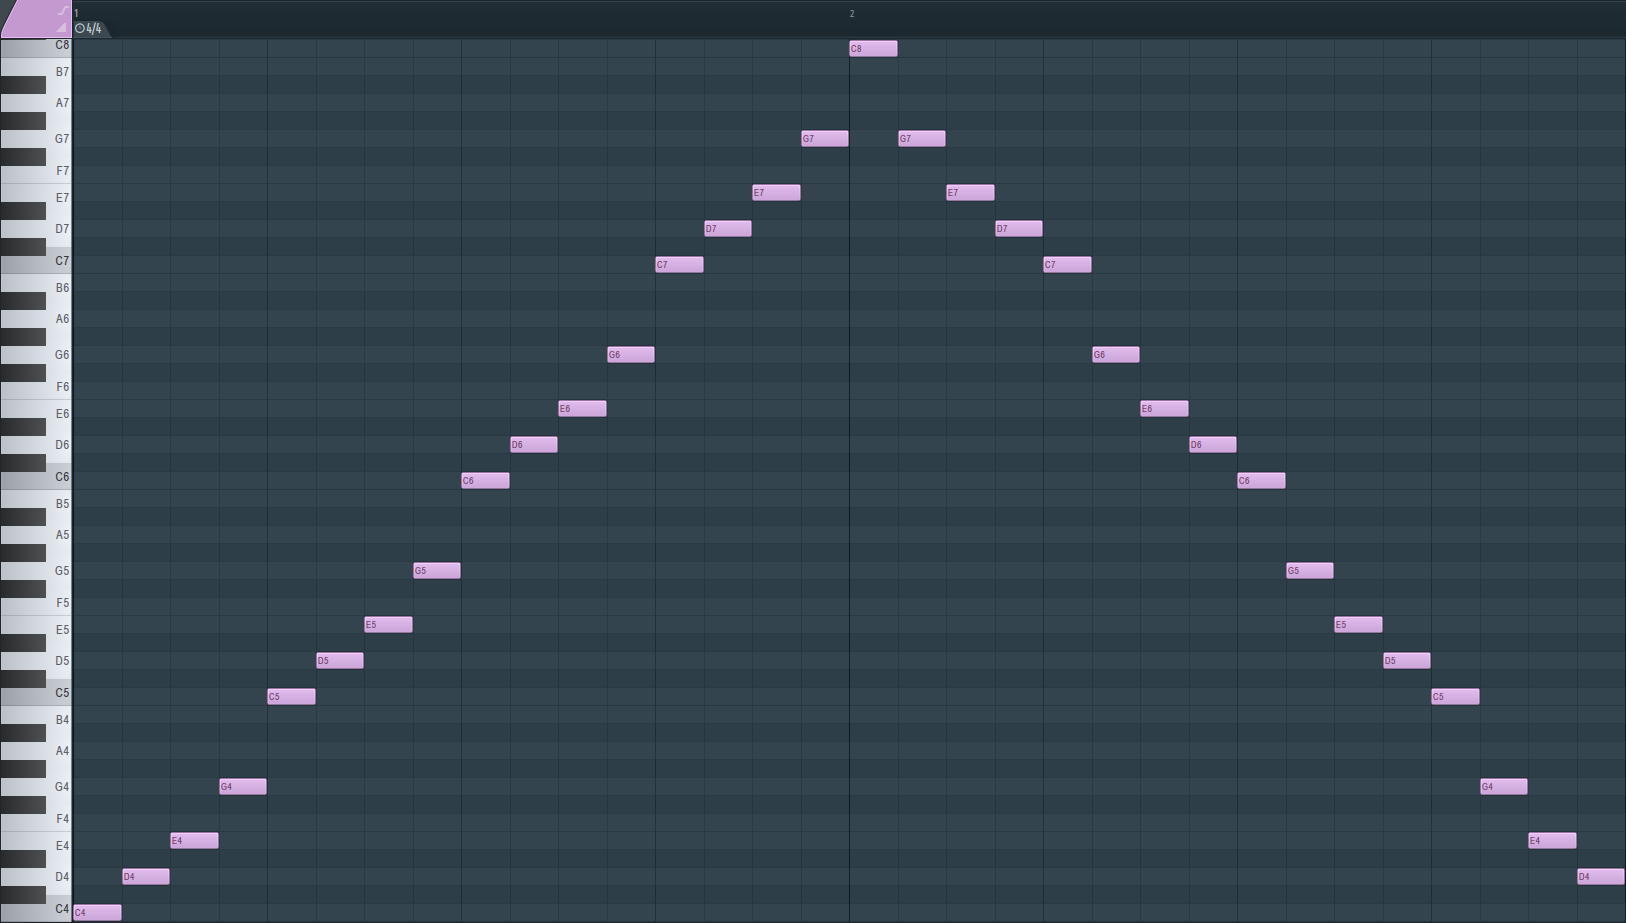
\includegraphics[width=.95\linewidth]{images/Noten_A.png}
	\caption{Notenabfolge A}
	\label{NotenabfolgeA}
\end{figure}
Unser Dokument sieht bisher wie folgt aus:

\medskip

\lstinputlisting[framexleftmargin=8mm, frame=shadowbox, rulesepcolor=\color{blue}, numbers=left]{codes/PreludeKanal1_1.txt}

%\medskip
\clearpage

Wir füllen nun den 1. Kanal mit Noten. Im Bild sehen wir die Noten der ersten 2 Takte (engl. Bar. Ein Takt besteht bei einem 4/4-Takt aus 4 Viertelnoten, bei einem 3/4-Takt aus 3 Viertelnoten usw.) Die einzelnen Noten sind daher 16tel Noten. Die gezeigte Notenfolge nennen wir zur Veranschaulichung A. \\
Nun schreiben wir die Noten in den Kanal: c16 d16 e16 g16

\bigskip

Ein Wechsel in einen anderen Oktavraum können wir entweder durch erneutes setzen des o Befehls erreichen oder durch > (Wechsel in den nächst höheren Raum) bzw. < (Wechsel in den nächst niedrigeren Raum). Die bevorzugte Variante sollte > und < sein. Der Vorteil liegt darin, dass > und < den Oktavraum in Relation zum vorherigen angeben, während der o Befehl einen absoluten Wert festlegt. Durch das Ändern der ersten Oktave eines Kanals bewegen sich daher alle Noten mit dem gleichen Oktavabstand mit, während bei der Nutzung von o Befehlen jede Oktave manuell geändert werden müsste. \\
Für die ersten zwei Takte ergibt sich dadurch:

\medskip

\lstinputlisting[framexleftmargin=8mm, frame=shadowbox, rulesepcolor=\color{blue}, numbers=left]{codes/PreludeKanal1_2.txt}

\medskip

Leerzeichen und Zeilenumbrüche werden von AddMusicK nicht interpretiert und dienen nur der besseren Übersicht.
Mit einem Semikolon ; können Kommentare eingefügt werden. Ein Kommentar wird von AddMusicK vollständig ignoriert und nimmt keinen Platz im Arbeistspeicher ein.

\subsubsection{Standardlänge}

Mit dem l Befehl (length) kann die Standardlänge von Noten und Pausen definiert werden, also der Länge, die von AddMusicK angenommen wird, wenn keine Länge hinter einer Note bzw. Pause steht (normalerweise 1). Da alle Noten in diesem Kanal aus 16tel Noten bestehen, können wir den Code mit l16 übersichtlicher gestalten. Hierbei sei gesagt, dass der l Befehl nicht die Größe des Songs verringert, sondern nur der Übersicht dient. Das Textdokument sieht nun folgendermaßen aus:

%\medskip
\clearpage

\lstinputlisting[framexleftmargin=8mm, frame=shadowbox, rulesepcolor=\color{blue}, numbers=left]{codes/PreludeKanal1_3.txt}

\medskip

Im folgenden Bild sehen wir die Noten der nächsten 2 Takte. Die Notenabfolge nennen wir B. Zu Übungszwecken soll diese selbst geschrieben werden.

%\newpage

\begin{figure}[htbp] \centering
	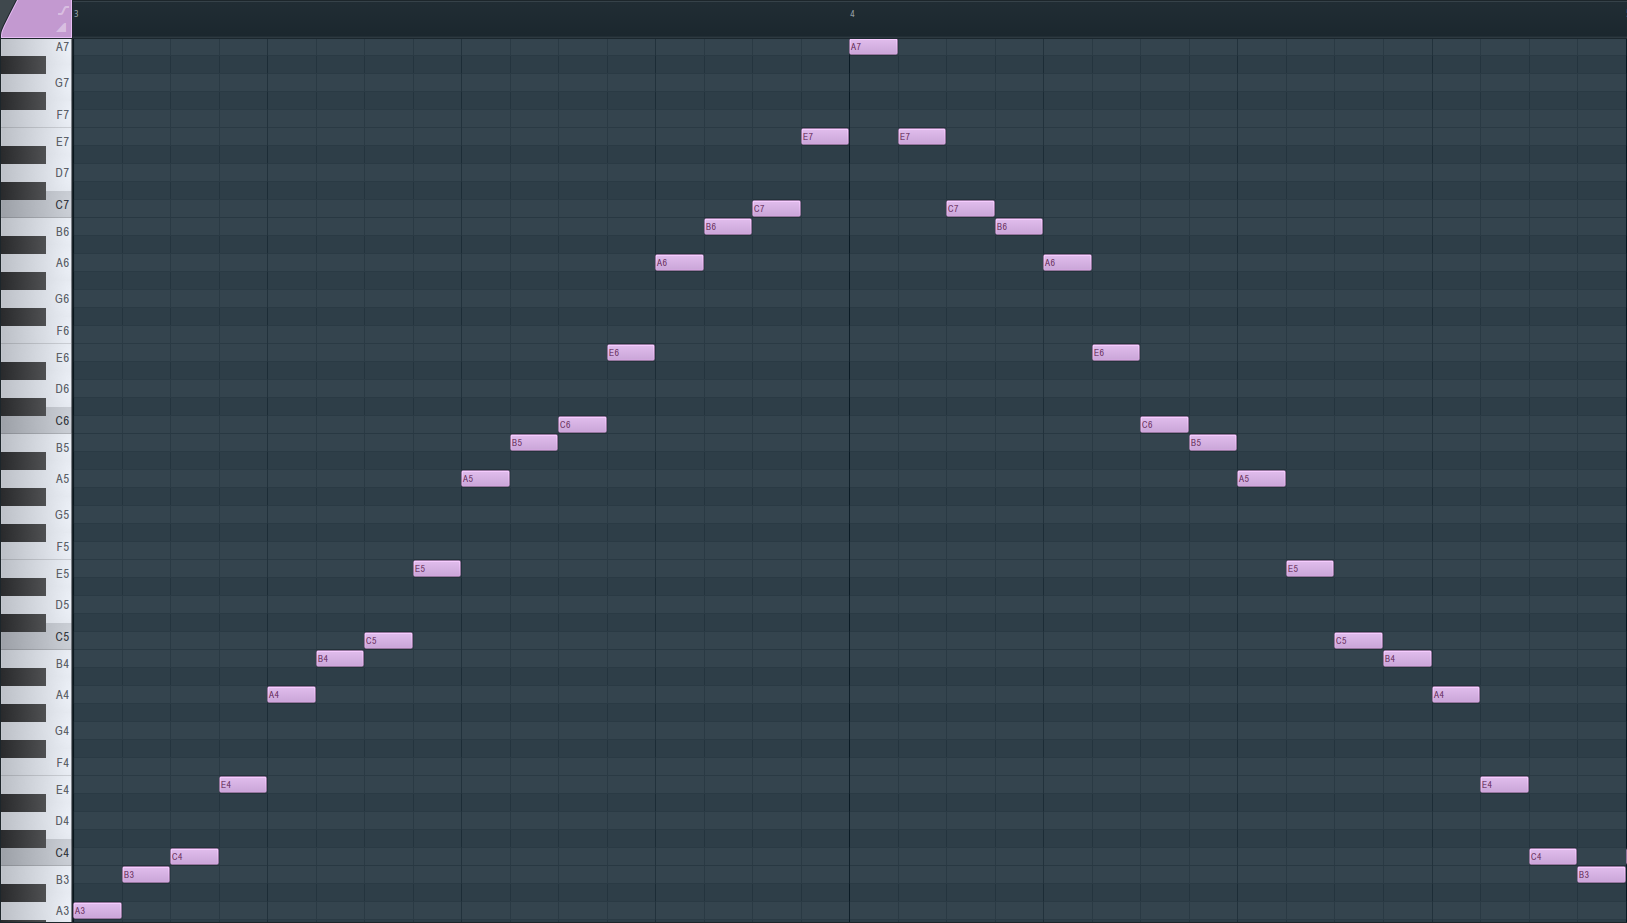
\includegraphics[width=.95\linewidth]{images/Noten_B.png}
	\caption{Notenabfolge B}
	\label{NotenabfolgeB}
\end{figure}

Wenn alles geklappt hat, sieht der Song nun wie folgt aus:

\medskip

\lstinputlisting[framexleftmargin=8mm, frame=shadowbox, rulesepcolor=\color{blue}, numbers=left]{codes/PreludeKanal1_4.txt}

\medskip

Dies ist eine gute Gelegenheit, um den Song Probe zu hören.
Dafür öffnen wir \textit{AMKGUI.exe}, scrollen im unteren Fenster Local Songs so weit nach unten wie es geht und klicken auf den letzten Song. Als nächstes gehen wir auf \textit{Add new Song} und wählen unsere Textdatei aus. Diese sollte jetzt markiert sein. Als nächstes setzen wir den Haken bei \textit{Porter mode} und klicken auf \textit{Run}. AddMusicK erzeugt aus der Textdatei eine SPC Datei die automatisch abgespielt wird, sofern der SPC Player als Standardprogramm für SPC Dateien gesetzt wurde. Falls dies nicht der Fall ist, wird eine Fehlermeldung erscheinen und wir müssen die SPC manuell öffnen. Eine SPC Datei wird nach dem Porten automatisch im Ordner SPCs abgelegt.


\begin{figure}[htbp] \centering
	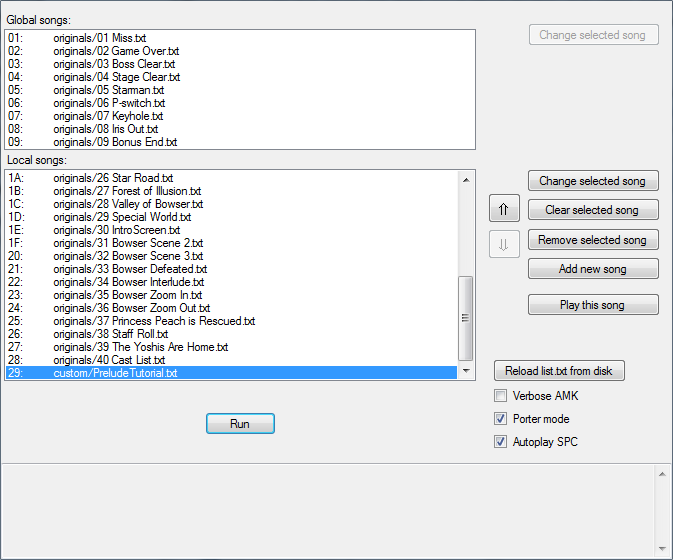
\includegraphics[width=.95\linewidth]{images/AMKGUI.png}
	\caption{AMKGUI.exe}
	\label{AMKGUI}
\end{figure}


Als nächstes kommen wieder Notenfolge A und B. Anstatt die Notenfolgen zu kopieren, benutzen wir ein neues Werkzeug und zwar Loops.

\subsubsection{Loops}
Jede Note die wir schreiben vergrößert den Song. Mit Loops können wir wiederkehrende Notenabfolgen zusammenfassen, einmalig speichern und aufrufen wann wir wollen.
Das Speichern eines Loops verbraucht zwar ebenso Speicherplatz, ist der Loop aber groß genug und wird mehrfach aufgerufen, kann man dadurch eine Menge Platz im Arbeitsspeicher sparen.
Hierbei sei gesagt, dass man auf keinen Fall extrem kurze oder gar nur einzelne Noten in einen Loop speichern sollte, falls diese nicht oft genug wiederholt werden, weil dies den umgekehrten Effekt hat und den Song vergrößert. \\
Es gibt 3 Arten von Loops: Normale Loops, Labeled Loops und Superloops. Wir verwenden hier einen normalen Loop. Dieser speichert alles was sich in eckigen Klammern [] befindet in einem Loop ab, eine Zahl dahinter gibt an, wie oft dieser Loop gespielt werden soll. Unsere Notenabfolge A B A B wird dadurch zu [A B]2


\lstinputlisting[framexleftmargin=8mm, frame=shadowbox, rulesepcolor=\color{blue}, numbers=left]{codes/PreludeKanal1_5.txt}

\medskip

Wichtig bei Loops im allgemeinen ist folgendes zu beachten: Ein sauberer normaler Loop hat immer gleich viele > und <. Dadurch ist sichergestellt, dass wir uns am Ende eines Loops in der gleichen Oktave befinden wie am Anfang des Loops. Ist dies nicht der Fall, laufen die Noten beim erneuten Durchlauf aus. Daher muss wie im Codebeispiel am Ende der Notenabfolge B ein > platziert werden.
Täten wir dies nicht, würde beim zweiten Durchlauf des Loops das erste C nicht in der zweiten Oktave beginnen, sondern in der ersten, weil das die letzte Oktave war in der wir uns befanden als das letzte b gespielt wurde.

\bigskip

Als nächstes kommen die Notenabfolgen C, D, E und F. Wer mag, kann diese zu Übungszwecken selbst schreiben, die Bilder dazu befinden sich im Anhang.

Der Song sieht nun wie folgt aus:

%\newpage
\medskip

\lstinputlisting[framexleftmargin=8mm, frame=shadowbox, rulesepcolor=\color{blue}, numbers=left]{codes/PreludeKanal1_6.txt}

\medskip

Diese gesamte Notenabfolge A B A B C D E F bzw. [A B]2 C D E F wird 3 mal hintereinander abgespielt. Es bietet sich daher an, einen weiteren Loop zu verwenden. Einen normalen Loop können wir aber nicht in einen anderen normalen Loop verschachteln. Dafür gibt es Superloops, gekennzeichnet durch doppelte Eckige Klammern [[]].
Dadurch wird unser Song zu [[ [A B]2 C D E F ]]3. \\
In eine weitere Ebene zu verschachteln ist nicht möglich, es können jedoch beliebig viele normale und labeled Loops parallel in einem Superloop zusammengefasst werden. \\
Nachdem der Superloop platziert wurde, sieht unser Song wie folgt aus:

\medskip

\lstinputlisting[framexleftmargin=8mm, frame=shadowbox, rulesepcolor=\color{blue}, numbers=left]{codes/PreludeKanal1_7.txt}

\medskip

Alle Noten für Kanal \#0 sind gesetzt. Wir können diesen Kanal nun weiter bearbeiten.

\subsubsection{Panning}
Panning (oder kurz Pan) bezeichnet die Aufteilung der Lautstärke auf unterschiedliche Lautsprecher. Der entsprechende Befehl in MML ist y. Gültige Werte liegen zwischen 0 und 20, dabei gilt: \\
y0 : 100\% Lautstärke auf rechten Lautsprecher \\
y20 : 100\% Lautstärke auf linken Lautsprecher \\
y10 : 50\% Lautstärke auf rechten und linken Lautsprecher (Standardwert) 

\bigskip

Panning hilft uns dabei, einen Song räumlicher klingen zu lassen. \\
Es ist auch möglich, Panning kontinuierlich zu ändern. Dafür verwenden wir unseren ersten Hex-Befehl.

\bigskip
Hex-Befehle erkennt man daran, dass diese immer mit einem \$ beginnen, gefolgt von einem zweistelligen Hexwert. Der Befehl für das so genannte Pan Fading ist \$DC \$XX \$YY, wobei XX und YY Hexwerte sind, die das Fading weiter beschreiben. \$XX gibt die Dauer des Prozesses an, \$YY gibt den Panning Wert an, auf den geändert werden soll. \\
Wir möchten in Kanal \#0 das Panning so haben, dass es mit 75\% links und 25\% rechts beginnt (y15) und nach einem Takt mit 75\% rechts und 25\% links aufhört (y5). Danach soll das Panning für den nächsten Takt den genau entgegengesetzten Verlauf haben, sodass wir nach insgesamt 2 Takten wieder bei y15 sind. Dieser Vorgang soll sich in Kanal \#0 durch den gesamten Song ziehen. \\
Als erstes müssen wir unseren Startwert festlegen, also y15. Danach kommt der erste Hexbefehl \$DC. Als nächstes kommt die Dauer. 1 Takt bzw. eine ganze Note als Hexwert ausgedrüct ist \$C0. Diesen Wert kann man entweder ausrechnen (siehe Ticks) oder in der entsprechenden Tabelle im Anhang nachschauen. Unser Zielwert ist 5.  Der erste Befehl um die Lautstärke vom linken zum rechten Lautsprecher zu verschieben ist somit fertig definiert:  \$DC \$C0 \$05.\\
Wollen wir wieder auf y15 zurück, machen wir dies mit \$DC \$C0 \$0F, wobei 15 als Hexwert \$0F ist. Wer Probleme beim Umrechnen von Dezimalzahlen zu Hexwerten hat kann auch einen Taschenrechner benutzen und diesen auf Programmierer einstellen.
Die beiden Befehle schreiben wir nun abwechselnd nach jeweils einem Takt in den ersten Kanal. \\
Der Song sollte nun folgendermaßen aussehen:

\medskip

\lstinputlisting[framexleftmargin=8mm, frame=shadowbox, rulesepcolor=\color{blue}, numbers=left]{codes/Panning.txt}

\medskip

\subsubsection{Instrumente setzen}
Instrumente werden mit @ ausgewählt, gefolgt von einer Nummer. Mit 0 - 18 und 21 - 29 werden Instrumente bestehend aus Super Mario World Samples mit bestimmten Voreinstellungen angewählt. Instrumentnummern 30+ sind Instrumente, die in \#instruments definiert wurden. Dabei ist es egal, ob die dafür verwendeten Samples aus SMW kommen oder eigene -- sogenannte custom Samples -- verwendet werden. Das Standardinstrument ist @0 was automatisch gewählt wird, wenn in einem Kanal kein Instrument platziert wird.
Eine vollständige Liste der SMW Samples befindet sich im Anhang. \\
Zum Testen empfehle ich in Zeile 7 verschiedene Instrumente auszuwählen, z.B. @2, @3 oder @5 und diese anzuhören. \\
Das Sample des Standardinstruments @0 soll beibehalten werden, allerdings ändern wir dessen ADSR Werte (Attack, Decay, Sustain, Release). Dafür gibt es zwei Möglichkeiten. Entweder mit dem Hex-Befehl \$ED oder mit dem Spezial Befehl \#instruments. Wir verwenden letzteres, die genaue Funktionsweise und Unterschiede werden im Kapitel ADSR weiter erläutert.

\bigskip

Wir definieren uns nun ein neues Instrument auf Basis des Samples von @0 mit anderen Eigenschaften.
Da es sich hierbei um einen Spezial Befehl handelt, kommt dieser in den ersten Teil des Dokuments. Das neu definierte Instrument rufen wir mit @30 auf.

\medskip

\lstinputlisting[framexleftmargin=8mm, frame=shadowbox, rulesepcolor=\color{blue}, numbers=left, lastline=12]{codes/Instrument30.txt}

\medskip

Wir bauen unseren Song nun weiter. Im Folgenden Bild sehen wir einige Begleitakkorde. 

\begin{figure}[htbp] \centering
	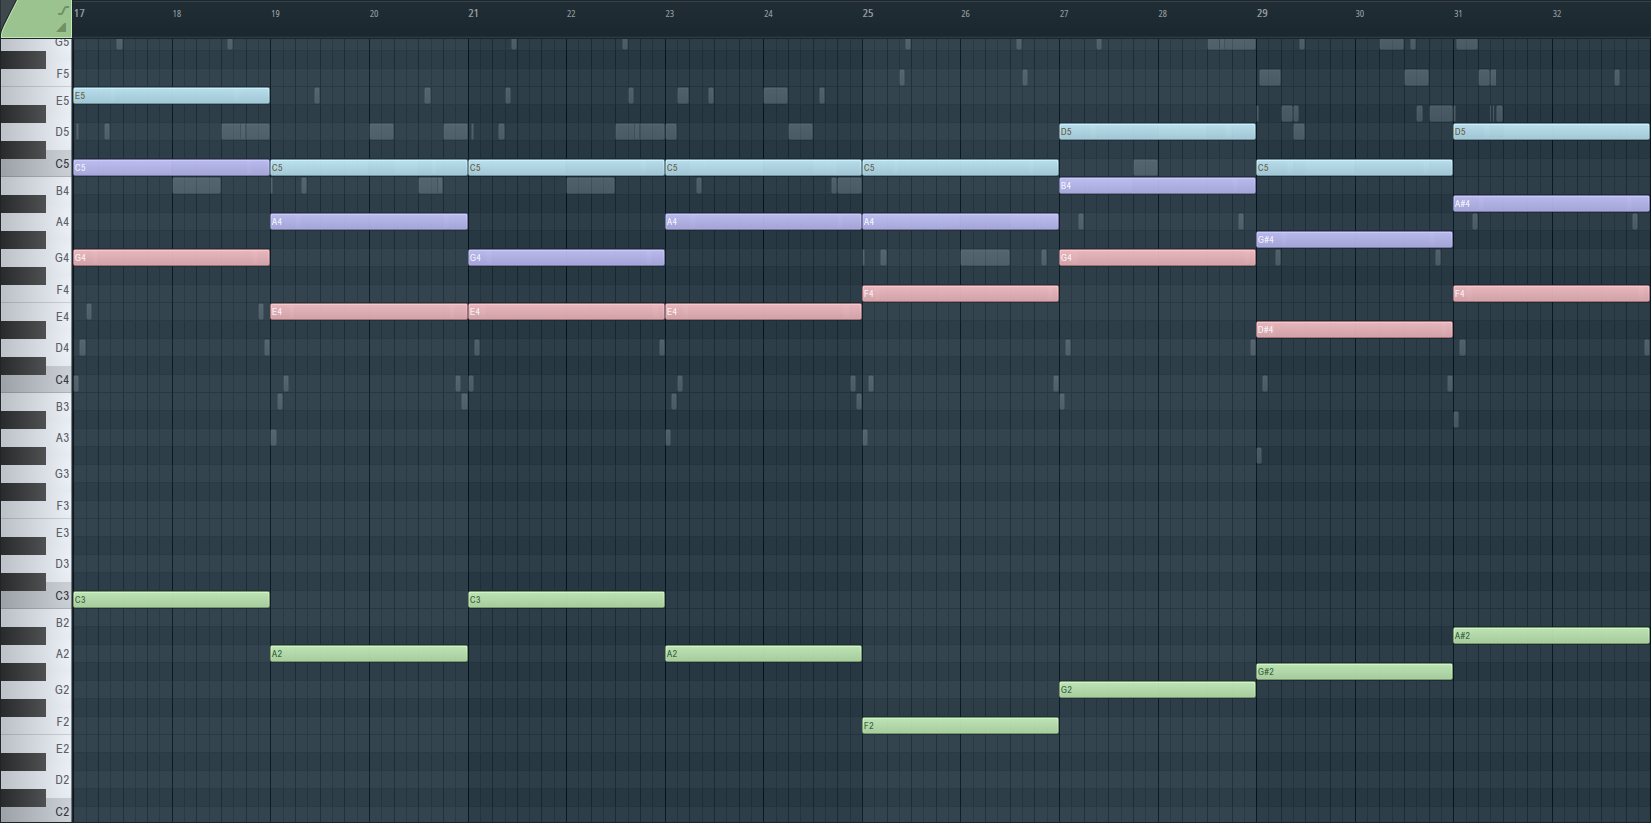
\includegraphics[width=.95\linewidth]{images/Strings.png}
	\caption{Kanal 2 bis 5}
	\label{NStrings}
\end{figure}

Der erste Kanal ist vollständig und wird nicht weiter bearbeitet. Parallel zum 1. Kanal folgt nach 16 Takten eine Begleitung. Die Noten erstrecken sich jeweils über 2 Takte und haben deshalb einen Notenwert
von 1\textasciicircum1. Pro Kanal kann aber nur eine Note gleichzeitig platziert werden. Deshalb brauchen wir für diese Begleitung 4 Kanäle. Die Noten ordnen wir auf die Kanäle wie folgt zu:

\bigskip

Kanal \#1 blaue Noten, angefangen bei Oktave 5 \\
Kanal \#2 lila Noten, angefangen bei Oktave 5 \\
Kanal \#3 rote Noten, angefangen bei Oktave 4 \\
Kanal \#4 grüne Noten, angefangen bei Oktave 3

\bigskip

Die Begleitung soll außerdem ein weiteres mal wiederholt werden, sodass sie von Takt 17 bis 32 und dann nochmal von Takt 33 bis 48 gespielt wird. Zu Übungszwecken sollen diese 4 Kanäle selbst geschrieben werden.

\bigskip

Kanal \#1 bis \#4 sollten wie folgt aussehen: 

\medskip

\lstinputlisting[framexleftmargin=8mm, frame=shadowbox, rulesepcolor=\color{blue}, numbers=left, firstline=41]{codes/Instrument30.txt}

\medskip

Als nächstes definieren wir uns ein neues Instrument auf Basis des Samples von @1 für die vier Kanäle.
Wir fügen es in \#Instruments ein und können es mit @31 auswählen.
Hierbei ist auf die Reihenfolge der Instrumente zu achten, weil diese die Nummerierung vorgibt. Das @30 und @31 hinter den Semikolons sind nur Kommentare.

\medskip

\lstinputlisting[framexleftmargin=8mm, frame=shadowbox, rulesepcolor=\color{blue}, numbers=left, firstline=3, lastline=7]{codes/Instrument31.txt}

\medskip

Wir weisen allen Noten in Kanal \#1, \#2, \#3 und \#4 das neue Instrument mit @31 zu und hören den Song probe. Nach ungefähr 47 Sekunden setzt unsere Begleitung ein.

\subsubsection{Lokale Lautstärke}
Wie wir bereits gelernt haben, wird mit dem w Befehl die globale Lautstärke des Songs eingestellt. Mit dem v Befehl können Noten der einzelnen Kanäle zusätzlich individuell eingestellt werden. Auch hier liegt der Wertebereich zwischen v0 und v255. \\
Die Noten in den vier neuen Kanälen stellen wir etwas leiser ein, indem wir in jeden der Kanäle ein v220 schreiben. Zusätzlich dazu stellen wir das Panning ein, damit die Akkorde ein wenig auf den Lautsprechern aufgeteilt werden. \\
Die Kanäle mit der Begleitung sehen nun so aus: \\

\medskip

\lstinputlisting[framexleftmargin=8mm, frame=shadowbox, rulesepcolor=\color{blue}, numbers=left, firstline=44, lastline=62]{codes/PreludeTutorial.txt}

\medskip

Als letztes fehlt noch ein weiteres Instrument was in Kanal \#5 zum Einsatz kommen soll. Wir definieren es wie folgt:

\medskip

\lstinputlisting[framexleftmargin=8mm, frame=shadowbox, rulesepcolor=\color{blue}, numbers=left, firstline=3, lastline=8]{codes/PreludeTutorial.txt}

\medskip

Da Kanal \#5 extrem kurze Noten enthält die nur schwer ablesbar sind, kann unser letzter Kanal der Vollständigkeit halber einfach aus dem Codebeispiel übernommen werden. \\
Wie wir in Zeile 8 und 9 sehen, kann ein Instrument in einem Kanal beliebig oft gewechselt werden.
Das ist auch notwendig für komplexere Songs um mehr als 8 Instrumente in einem Song benutzen zu können.

\newpage

\lstinputlisting[framexleftmargin=8mm, frame=shadowbox, rulesepcolor=\color{blue}, numbers=left, firstline=64, lastline=73]{codes/PreludeTutorial.txt}

\medskip

An dieser Stelle wird an dem Song nicht mehr weiter geschrieben. Er soll aber dennoch abgespeichert werden, da wir in späteren Kapiteln diesen für andere Beispiele benutzen werden.
\newpage
\section{Song aus Midi konvertieren}

Bisher haben wir manuell einen Song in einem Texteditor geschrieben. Für komplexere und längere Songs eignet sich das Konvertieren aus einer MIDI Datei. Ein Konverter übernimmt allerdings nur einen Teil unserer Arbeit. Die MIDI Datei muss vor dem Konvertiervorgang aufbereitet und das Ergebnis weiterhin im Texteditor bearbeitet werden.
\subsection{Vergleich der Konverter}
In diesem Kapitel werden drei Konverter vorgestellt, die alle Vor- und Nachteile mit sich bringen. Dabei handelt es sich um PetiteMM von gocha und loveemu, MIDI2MML von NeutronCat und mmltk von Nobody-86.
\subsubsection*{PetiteMM}
PetiteMM ist der mit Abstand älteste der drei Konverter mit einem simplen GUI.

\subsubsection*{Vorteile}
\begin{itemize}
	\item Java Programm lässt Benutzung auf Windows und MacOS zu
	\item Schneller Konvertiervorgang
	\item Konvertiert fast fehlerfrei
\end{itemize}

\subsubsection*{Nachteile}
\begin{itemize}
	\item Keine schöne MML Code Formatierung
\end{itemize}

\subsubsection*{MIDI2MML}
MIDI2MML ist ein neuerer Konverter aus Ende 2020.

\subsubsection*{Vorteile}
\begin{itemize}
	\item Benutzerfreundliches GUI
	\item Schneller Konvertiervorgang
	\item Schöne MML Code Formatierung
	\item Überlappende Noten werden über 8 Kanäle hinaus in separate Kanäle abgespeichert
	\item MIDI Events sind einsehbar
\end{itemize}

\subsubsection*{Nachteile}
\begin{itemize}
	\item C\# Programm, daher nur auf Windows zu benutzen
	\item Konverter interpretiert gewisse Notenwerte falsch
	\item Einige Notenwerte werden nicht intuitiv dargestellt.
\end{itemize}

\subsubsection*{mmltk}
mmltk ist ein weiterer neuerer Konverter aus Ende 2020, in Python geschrieben und als einziger Konsolenbasiert.

\subsubsection*{Vorteile}
\begin{itemize}
	\item Schöne MML Code Formatierung
	\item Überlappende Noten werden über 8 Kanäle hinaus in separate Kanäle abgespeichert
	\item Einziger Konverter der konstant fehlerfrei konvertiert
	\item Kann zusätzlich MML in eine MIDI Datei zurück konvertieren (experimentell)
\end{itemize}

\subsubsection*{Nachteile}
\begin{itemize}
	\item Programm momentan nur auf Windows zu benutzen
	\item Langsamer Konvertiervorgang
	\item Einmalige Installation aufwändiger als bei den anderen Konvertern
\end{itemize}

Da mmltk bei weitem das beste Ergebnis liefert, empfehle ich an dieser Stelle den einmaligen Mehraufwand der Installation.

\subsection{Installation und Benutzung von mmltk}
mmltk basiert auf Python, der erste Schritt ist also Python zu installieren.
Python kann hier heruntergeladen werden: \href{https://www.python.org/downloads/}{https://www.python.org/downloads/}

\bigskip

Als nächstes öffnen wir die Konsole und geben python -{}-version ein um zu testen, ob Python korrekt installiert wurde. Daraufhin sollte die Konsole mit der Versionsnummer von Python antworten.

\begin{figure}[htbp] \centering
	\includegraphics[width=.95\linewidth]{images/Python.png}
	\caption{Versionsnummer von Python aufrufen}
	\label{Python}
\end{figure}

mmltk benötigt 3 weitere Pakete die wir nun installieren und zwar mido, numpy und pandas.
Um die Pakete jeweils zu installieren, geben wir nacheinander

\bigskip

python -m pip install mido \\
python -m pip install numpy \\
python -m pip install pandas

\bigskip

ein. Ab jetzt können wir mmltk benutzen. Es kann unter \href{https://gitlab.com/Nobody-86/mmltk}{https://gitlab.com/Nobody-86/mmltk} heruntergeladen werden. \\
Nachdem wir die Datei an einem Ort unserer Wahl entpackt haben, öffnen wir wieder die Konsole.
Wir navigieren mit dem Befehl cd zu dem Verzeichnis, in dem mmltk.py liegt. Mit dem Befehl

\bigskip

python mmltk.py -i  \dq MIDINAME.mid\dq{} -o \dq MMLNAME.txt\dq{}

\bigskip

wird eine Midi in ein MML Dokument konvertiert, die im selben Verzeichnis liegt wie mmltk.py. \\
Alternativ kann auch der Pfad angegeben werden, falls die Midi nicht im selben Verzeichnis liegt wie mmltk.py. Tipp: Per Drag \& Drop wird automatisch der Dateipfad in die Konsole geschrieben.

\begin{figure}[htbp] \centering
	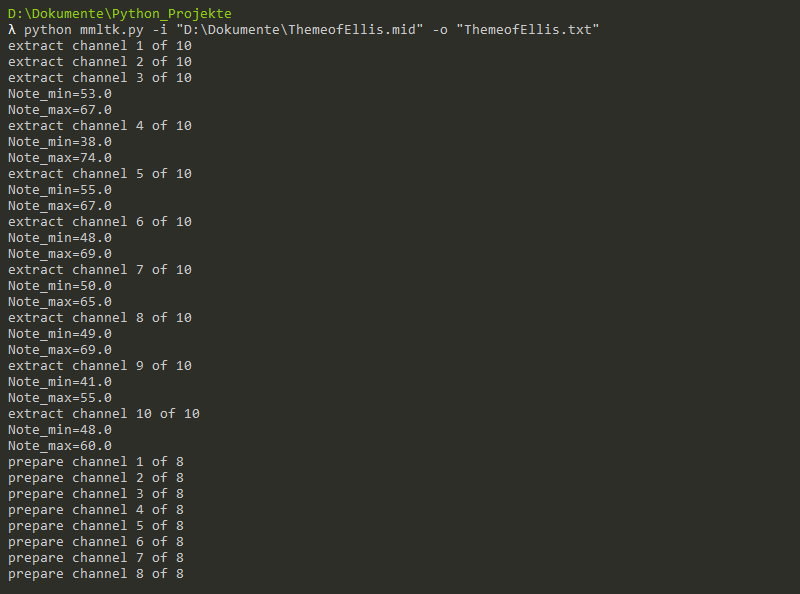
\includegraphics[width=.95\linewidth]{images/mmltk.png}
	\caption{MIDI mit mmltk in ein Textdokument mit MML konvertieren}
	\label{mmltk}
\end{figure}

\subsection{Midi aufbereiten und konvertieren}

Neben dem Konverter wird zusätzlich noch ein Programm benötigt, mit dem MIDIs (in einer Piano Roll) bearbeitet werden können. Beispiele dafür sind FL Studio, LMMS oder Anvil Studio. Die Trial Version von FL Studio reicht für unsere Zwecke vollkommen aus und beschränkt uns hinsichtlich des Arbeitens an Midi Dateien nicht. In diesem Tutorial benutze ich FL Studio und beschreibe den allgemeinen Umgang damit. \\
Wir öffnen eine beliebige MIDI Datei mit FL Studio, am einfachsten geht dies, indem die Datei per Drag \& Drop in das offene Programm gezogen wird. Wichtig hierbei ist, dass FL Studio nur MIDI Dateien mit der Endung .mid und nicht .midi öffnen kann. \\
Das folgende Fenster wird sich öffnen: 

\begin{figure}[htbp] \centering
	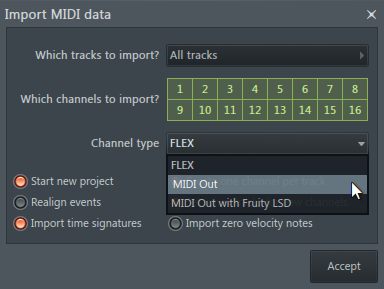
\includegraphics[width=.45\linewidth]{images/ImportMidi.png}
	\caption{MIDI mit FL Studio öffnen}
	\label{ImportMidi}
\end{figure}

Wir stellen den Channel type auf \textit{MIDI Out}. Falls zur MIDI Datei eine Soundbank in Form einer DLS (Downloadable Sound) Datei vorliegt, kann auch \textit{MIDI Out with Fruity LSD} ausgewählt werden. \textit{FLEX} sollte vermieden werden, besonders wenn man nur die Trial Version besitzt und keine FL Studio Projekte öffnen kann. FLEX Kanäle können notfalls auch im Nachhinein noch durch MIDI Out Kanäle ersetzt werden. \\
Als nächstes muss der MIDI Port geändert werden und zwar auf den gleichen, den auch die MIDI Out Kanäle verwenden (standardmäßig auf 0) Mit F10 öffnen sich die MIDI Settings, dort stellen wir den Port auf 0.

\bigskip

\begin{figure}[htbp] \centering
	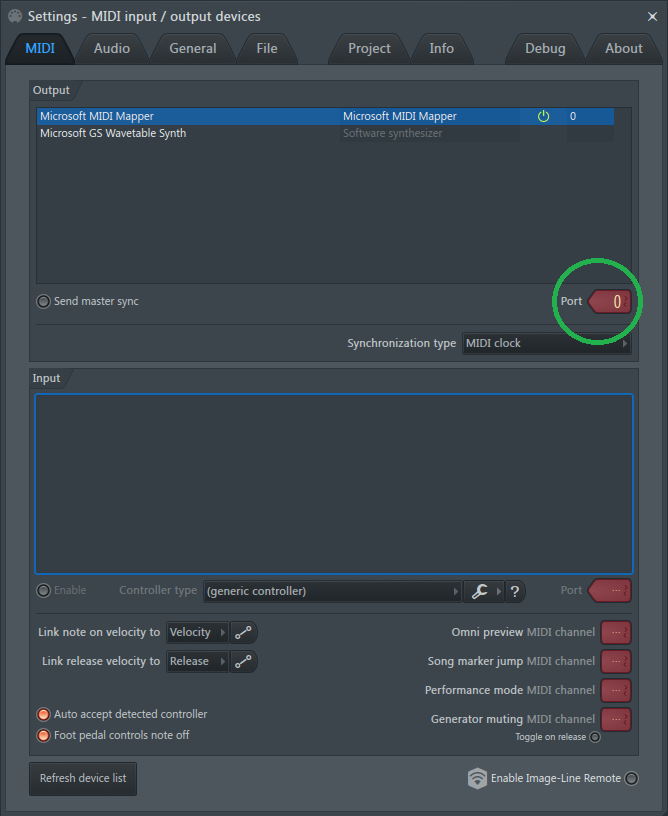
\includegraphics[width=.63\linewidth]{images/MIDIPort.png}
	\caption{MIDI Port wählen}
	\label{MIDIPort}
\end{figure}

Zusätzlich kann über den Reiter \textit{Project} die Timebase auf 48 PPQ eingestellt werden. Dadurch sind alle Noten und Pausen im richtigen Maß quantisiert, wodurch garantiert ist, dass die zeitliche Auflösung nie überschritten wird.

\bigskip

Ab jetzt sind alle Vorkehrungen getroffen und die MIDI Datei kann nach den bereits erwähnten Einschränkungen bearbeitet werden (pro Kanal nur eine Note gleichzeitig, maximal 8 Kanäle, Noten zwischen den Oktaven o1c bis o6a).
Zusätzlich sollte darauf geachtet werden, welche Noten in den Kanälen 7 und 8 liegen. Kanal 8 ist in SMW hauptsächlich für den Sprung Soundeffekt reserviert (und einige weitere die aber eher selten benutzt werden), Kanal 7 für die restlichen Soundeffekte. Das hat zur Folge, dass vor allem lange Noten und Noten, die für eine markante Melodie zuständig sind, nicht in diesen beiden Kanälen untergebracht werden sollten. Jedes mal wenn ein Soundeffekt in SMW abgespielt wird, werden die Noten des entsprechenden Kanals stumm geschaltet. \\
Die vollständigen Listen aller Soundeffekte befinden sich in den Ordnern 1DF9 (Kanal 7) und 1DFC (Kanal 8).

\bigskip

Entspricht die MIDI Datei den Anforderungen, sollte das Projekt als .mid exportiert werden falls man nicht die Trial Version von FL Studio besitzt, weil man keine Projektdateien öffnen kann, MIDI Dateien aber schon (wie wir offensichtlich gesehen haben). \\
Hier sei noch einmal gesagt, dass man darauf achten soll, nicht FLEX zu benutzen, da es passieren kann, dass die exportierte MIDI Datei keine Noteninformationen enthält und alle Arbeiten verloren gehen.

\subsection{Einführung FL Studio}

Ein vollständiges Tutorial zu FL Studio würde bei weitem den Rahmen sprengen, es werden jedoch auf die Grundfunktionen eingegangen die ausreichen, um MIDI Dateien zu bearbeiten. Abbildung \ref{FLStudio} zeigt das Programm in mehrere Abschnitten unterteilt. Dabei  handelt es sich um:


\begin{itemize}
	\item 1. Channel Rack
	\item 2. + 3. Playlist
	\item 4. Play/Pause
\end{itemize}


\begin{figure}[htbp] \centering
	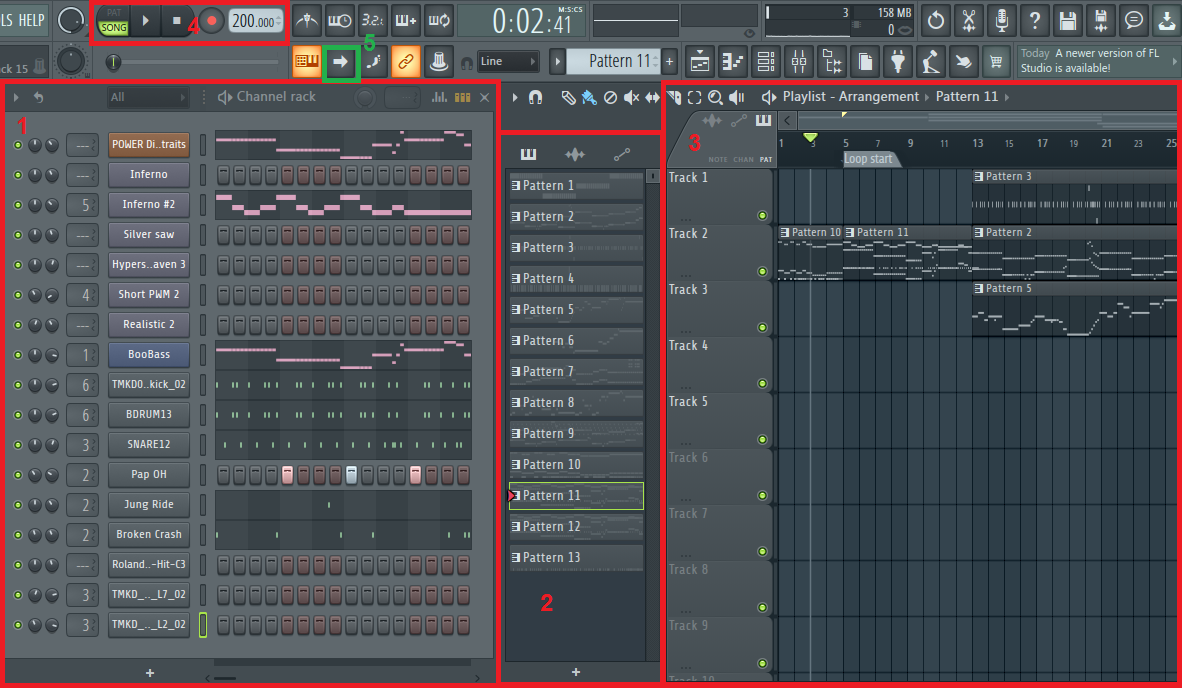
\includegraphics[width=.95\linewidth]{images/FLStudio.png}
	\caption{FL Studio Übersicht}
	\label{FLStudio}
\end{figure}

\subsubsection*{Channel Rack}

Im Channel Rack (F6) arbeiten wir die meiste Zeit. Hier befinden sich Kanäle, die entweder aus einem einfachen Sample oder einem VST (Virtual Studio Technology) Plugin bestehen. Jeder Kanal kann Noten beinhalten (im Falle eines Automation Clips ein Steuersignal). \\
Mit dem grünen Punkt Links vor jedem Kanal kann dieser Stumm geschaltet werden. Der linke Regler ist für das Panning (Lautstärkeverteilung auf Lautsprechern) und der rechte für die Lautstärke des Kanals zuständig. Das Feld daneben kann mit einer Zahl besetzt werden. Diese gibt an, welchen Platz der Kanal im Mixer (F9) belegen soll, um dort weiter mit Effekten wie Reverb etc. bearbeitet zu werden. Da wir nur mit MIDI arbeiten, kann sowohl dieses Zahlenfeld, als auch der Mixer ignoriert werden. \\
Mit einem Linksklick auf einen Kanal öffnen wir diesen. Je nachdem, was sich dort befindet, öffnen sich entweder der Plugin Editor oder die Sample bzw. Instrument Settings. Mit einem Klick auf den kleinen Pfeil in der oberen linken Ecke öffnet sich ein Menü, worüber man bei Plugins  beispielsweise Presets (also Voreinstellungen) laden kann. (Im Falle von MIDI OUT können so voreingestellt CC's (Continuous Controller) von Synthesizern geladen werden. Wie man MIDI Controller auch selbst anlegt wird später erklärt.) \\
Klicken wir neben den kleinen Pfeil auf das Zahnradsymbol, öffnet sich eine weitere Leiste. Dort befinden sich neben dem grünen Mute Knopf, dem Panning und Volume Regler noch ein Pitch Regler (den wir u.a. für Pitch Slides ausnutzen können).

\bigskip

Mit einem Rechtsklick auf den Kanalnamen haben wir weitere Optionen. Die wichtigsten hierbei sind \textit{Insert} bzw. \textit{Replace}, womit ein Kanal ersetzt bzw hinzugefügt werden kann (Funktioniert auch über das + am unteren Rand des Channel Racks) und die Piano Roll (oder auch F7, wenn der Kanal ausgewählt wurde). In Abbildung \ref{Channel} ist dargestellt, wie ein neuer MIDI Out Kanal hinzugefügt werden kann.


\begin{figure}[htbp] \centering
	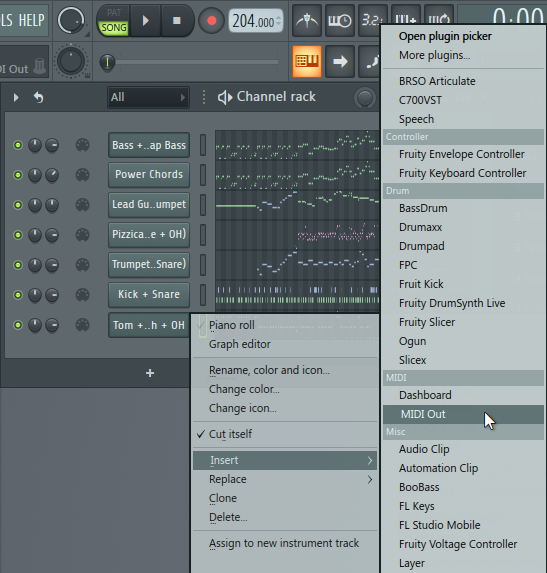
\includegraphics[width=.70\linewidth]{images/Channel.png}
	\caption{Channel einfügen}
	\label{Channel}
\end{figure}


Klickt man auf das schmale Select Feld (bekommt eine grüne Umrandung) ohne auf den Kanal geklickt zu haben (nicht dunkel unterlegt), kann mit der Tastenkombination Alt + Pfeiltasten ein Kanal verschoben werden.

\bigskip

Rechts neben dem Select Feld befindet sich der Step Sequencer bzw. eine Vorschau der Piano Roll. Mit den Standardeinstellungen hat der Step Sequencer einen 4/4 Takt, bestehend aus 16 16tel Noten. Den Step Sequencer verwendet man in der Regel nur mit Drum / Percussion Samples, da im Step Sequencer jede Note ein o5c ist. Die Piano Roll hingegen wird verwendet, um Noten in einen Kanal zu platzieren.

\subsubsection*{Playlist}

Als nächstes betrachten wir die Playlist. Der linke Bereich beinhaltet eine Liste an Pattern (Mustern), die im rechten Bereich der Playlist platziert werden können. In Abbildung \ref{FLStudio} besteht das Pattern 11 aus den Notenabfolgen, die im Channel Rack links daneben zu sehen sind. Wir können ein neues (leeres) Pattern über das + am unteren Fensterrand hinzufügen oder mit dem Feld Pattern über der Playlist (dort ist es auch möglich, ein Pattern zu kopieren, falls man ein ähnliches Muster haben möchte aber nur leicht bearbeitet werden soll)
Wir können so aus vielen kleinen Pattern Schnipseln einen Song bauen. \\
Es ist auch möglich, einen Song ohne Playlist zu bauen, indem sich der gesamte Song in nur einem Pattern befindet (was automatisch der Fall ist, wenn man eine MIDI Datei mit FL Studio öffnet).

\bigskip

In Feld 4 befinden sich die Play/Pause, Stop und Aufnahme Buttons. Außerdem kann über \textit{PAT} (orange) bzw \textit{SONG} (grün) bestimmt werden, ob das ausgewählte Pattern oder die Playlist abgespielt werden soll. \\
Rechts daneben befindet sich die BPM Anzeige, die das Tempo bestimmt. Mit einem Rechtsklick auf diese kann über den Punkt \textit{Tap} im Rhythmus eines Songs getippt werden, um die BPM Zahl einfach zu bestimmen. \\

Mit dem in Abbildung \ref{FLStudio} grün markierten Feld 5 schaltet man das automatische scrollen während des Play Vorgangs ein bzw. aus. Ich bevorzuge kein Autoscroll.

\subsubsection*{Piano Roll}

Werfen wir einen Blick auf die Piano Roll, können wir diese auch in mehrere Bereiche aufteilen. Im Hauptbereich können wir Noten platzieren und diese von der Länge anpassen, indem man am rechten Rand einer Note zieht (kann auch umgestellt werden). \\
Die senkrechten Striche im unteren Bereich geben die Lautstärke jeder einzelnen Note an. Diese kann dort verändert werden, es kann auch über das Feld \textit{Control} zwischen unterschiedlichen Parametern gewechselt werden (z.B. Panning). \\
Oben links in der Ecke befindet sich ein Pfeil, der eine Menge nützlicher Einstellmöglichkeiten
beinhaltet. Die wichtigsten sind \textit{Snap}, womit bestimmt wird, mit welchem Inkrement Notenlängen geändert und Note platziert werden und die \textit{Quantize} Funktionen unter Tools, womit markierte Noten auf eine vorgegebene Auflösung quantisiert werden können.

%\newpage

\begin{figure}[htbp] \centering
	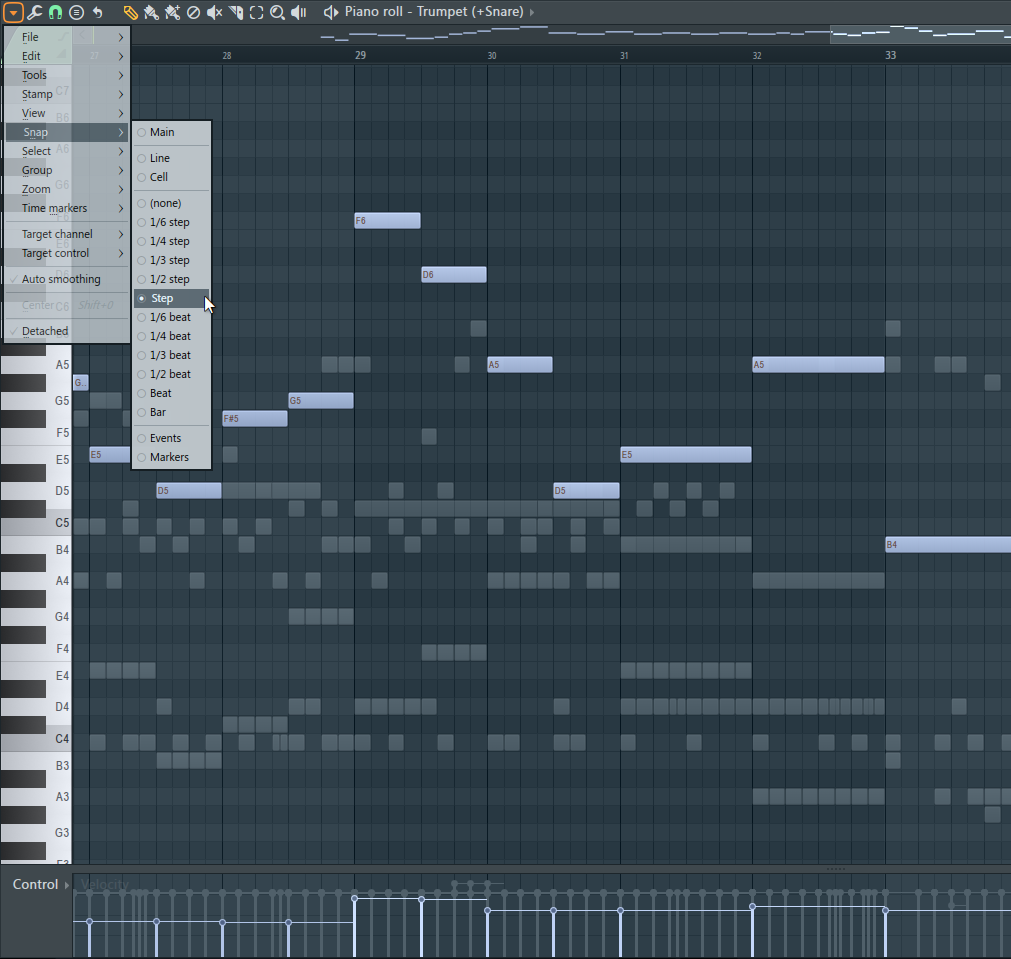
\includegraphics[width=.95\linewidth]{images/PianoRoll.png}
	\caption{Piano Roll Optionen}
	\label{PianoRoll}
\end{figure}

\bigskip

\subsubsection*{MIDI Out}

Erstellen wir einen MIDI Out Kanal wie in Abbildung \ref{Channel} und klicken auf den Kanal sehen wir die Plugin Settings. Die Channel Nummer ist das Äquivalent eines Kanals in MML, wobei die meisten MIDI/MML Konverter der Reihe und nicht nach Kanalnummer konvertieren. Eine Besonderheit ist der Kanal 10, dadurch wird die Piano Roll für diesen Kanal zu einem Drum Set, d.h. jede Note entspricht einem Drum bzw. Percussion Instrument. Rechts daneben kann im Feld \textit{Patch} ein MIDI Instrument für diesen Kanal ausgewählt werden. \\
Die Bank Felder können wir ignorieren, da wir keine Soundbanken verwenden werden. \\
Die Port Nummer muss die gleiche wie in Abbildung \ref{MIDIPort} sein, ansonsten fehlt die Soundausgabe.

\begin{figure}[htbp] \centering
	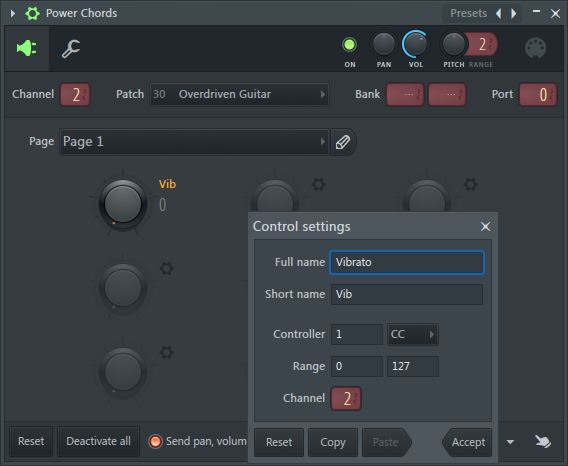
\includegraphics[width=.75\linewidth]{images/MIDIOut.png}
	\caption{geöffneter MIDI Out Kanal}
	\label{MIDIOut}
\end{figure}

Unten befindet sich ein Bereich mit 9 Reglern. Diese sind zunächst ohne Funktion, können von uns aber mit Controllern belegt werden. Dafür muss man mit einem Rechsklick auf das kleine Zahnrad neben dem Regler klicken um die Control Settings zu öffnen. \\
Hier kann man jedem Regler einen Namen und Funktion zuordnen. Wir benutzen Continuous Controller (CC) die je nach Nummer eine andere Funktion abdecken. Eine vollständige Liste der CC Nummern gibt es unter \href{https://nickfever.com/Music/midi-cc-list}{https://nickfever.com/Music/midi-cc-list} \\
CC Nummer 1 ist beispielsweise ein Controller für Vibrato. Die Range bestimmt einen Wertebereich, den man i.d.R. bei 0 bis 127 lassen sollte. \\
Die Letzte Channel Angabe bestimmt, welche Kanäle man mit genau diesem Regler ansteuern möchte.

\bigskip

An dieser Stelle sei gesagt, dass nicht alle CC's über MIDI Out selbst funktionieren (generell unterstützt nicht jedes Plugin oder Synthesizer alle Controller). Außerdem werden die Controller nicht mit in den MML Code konvertiert, sie sind aber dennoch nützlich als Referenz.

\bigskip

Ein nützliches Plugin ist BRSO Articulate, zu finden unter: \\ \href{https://www.syntheticorchestra.com/tools/articulate/}{https://www.syntheticorchestra.com/tools/articulate/} welches das MIDI Out Plugin von FL Studio ersetzt. Das Plugin kann sich selbst mit mehr Controllern ansteuern und es können Instrumente abhängig von der Farbe einer Note gesetzt werden (Noten Farben können in der Piano Roll geändert werden). Eine ausführliche Anleitung zum Plugin findet sich auf der Webseite. \\
VST Plugins lassen sich in FL Studio installieren, indem man die entsprechende .dll Datei des Plugins in den Ordner \textit{Plugins/VST/} oder \textit{Plugins/Fruity/Generators} legt und dann in FL Studio diese über die Plugin Database (links) aktiviert nachdem man sie über \textit{Options/Manage Plugins} gesucht hat.

\bigskip

Falls man nur die Trial Version von FL Studio besitzt und man keine Projekte öffnen kann, sind die Einsatzmöglichkeiten von BRSO Articulate begrenzt (genau auf eine Session).
\section{Instrumente und Samples}

In diesem Kapitel wird erklärt, was der Unterschied zwischen so genannten sampled und unsampled Songs ist, wie einzelne Instrumente definiert werden, was Sample Groups sind und wie wir eigene Samples erstellen und einbinden können. \\
Außerdem benötigen wir für das Kapitel folgende Programme:

\medskip

\begin{itemize}
	\item split700
	\item Audacity
	\item OpenMPT
	\item BRRPlayer
	\item C700 VST Plugin (optional, da split700 in diesem Fall die gleiche Aufgabe übernimmt. Trotzdem beides empfohlen)
\end{itemize}

\medskip


Unsampled Songs sind Songs, die ausschließlich Samples aus SMW benutzen. Ein Beispiel für ein unsampled Song ist der von uns erstellt Song aus Kapitel \ref{sec:ErstenSongSchreiben}. \\
Von sampled Songs ist die Rede, sobald mindestens ein custom Sample (ein Sample, dass aus einem anderen Spiel kommt oder selbst erstellt wurde) für den Song verwendet wird. \\
Unsampled Songs klingen oft nach SMW und haben den Vorteil, dass sie nur wenig Platz im Audio RAM einnehmen. Dafür ist man jedoch stark eingeschränkt in der Instrumentauswahl. Sampled Songs haben dieses Problem nicht, können aber schnell den gesamten Arbeitsspeicher belegen, weswegen besonders auf den Speicherplatz geachtet werden muss.

\subsection{Custom Samples}

Der SPC700 arbeitet mit so genannten .brr Samples (Bit Rate Reduction). Es gibt verschiedene Möglichkeiten an diese Samples zu gelangen:

\medskip

\begin{itemize}
	\item Ein Sample Pack herunterladen
	\item Samples aus einer SPC Datei extrahieren, z.B. mit split700, dem C700 Plugin oder SPC2MML
	\item Ein Sample aus einer .wav Datei selbst erstellen 
\end{itemize}

\medskip

Ein sehr umfangreiches Sample Pack ist samples of insanity von musicalman. Es ist hier verfügbar:
\href{https://bin.smwcentral.net/u/29022/soi-2019-07-12.zip}{https://bin.smwcentral.net/u/29022/soi-2019-07-12.zip}

\bigskip

Sollen Custom Samples für einen Song verwendet werden, müssen sich diese in einem Unterverzeichnis von AddmusicK/samples/ liegen. Am besten legt man für jeden Song einen eigenen Ordner für Samples an. Mit dem Spezial Befehl \#path weiß AddMusicK, in welchem Verzeichnis Samples gesucht werden sollen. \\
Wir fügen am Beispiel unseres Songs aus Kapitel \ref{sec:ErstenSongSchreiben} ein Custom Sample ein. Als erstes erstellen wir einen Ordner mit dem Namen \textit{Prelude} in AddmusicK/samples/. Danach kopieren wir uns das Sample Harp 2.brr, welches in samples of insanity/individual samples/other liegt und fügen es in den von uns zuvor erstellten Ordner \textit{Prelude} ein. Außerdem öffnen wir das beiliegende Textdokument \textit{!patterns.txt} worauf wir gleich noch zurückgreifen werden. \\
Jetzt öffnen wir wieder unseren Song und geben den Pfad mit \#path  \dq Prelude\dq{} an. Danach bestimmen wir mit \#samples\{\}, welche Samples aus dem Ordner benutzt werden sollen. Wir tragen neben dem Samplenamen noch eine Samplegroup ein die wir verwenden möchten, was entweder die Samplegroup \#default oder \#optimized ist, falls wir keine eigene erstellen. \\
AddMusicK legt im Hintergrund die Samplegroup \#default automatisch an wenn kein \#Samples\{\} Block vorhanden ist, weswegen wir bisher keine Samplegroup selber anlegen mussten.


\medskip

\lstinputlisting[framexleftmargin=8mm, frame=shadowbox, rulesepcolor=\color{blue}, numbers=left, firstline=1, lastline=9]{codes/Samples.txt}

\medskip

Als letztes definieren wir uns das neue Instrument. Wir ersetzen dafür das alte Instrument an die Position @30, indem  die gesamte Zeile gelöscht wird und dafür der Samplename plus den ersten 5 Hexwerten aus  \textit{!patterns.txt} die hinter  \textit{harp 2.brr} stehen. \\
Der Anfang des Songs sollte nun wie folgt aussehen:

\medskip

\lstinputlisting[framexleftmargin=8mm, frame=shadowbox, rulesepcolor=\color{blue}, numbers=left, firstline=1, lastline=17]{codes/Samples.txt}

\medskip


\subsection{Instrumente definieren}

Möglicherweise möchten wir ein Instrument in seinen Eigenschaften ändern oder haben gar keine Standardwerte, weil wir das Sample beispielsweise selbst erstellt haben. Was es mit den einzelnen Hexwerten auf sich hat wird im Folgenden erklärt.\\

\medskip
 
\lstinputlisting[framexleftmargin=8mm, frame=shadowbox, rulesepcolor=\color{blue}, numbers=left, firstline=13, lastline=13]{codes/Samples.txt}
 
\medskip

Als erstes wird entweder die Nummer des SMW Samples oder der Custom Sample Name angegeben, der definiert werden soll.
Danach beschreiben die Hexwerte der Reihe nach: \\
Attack und Decay (AD), Sustain und Release (SR), Gain, Pitch, Fine Pitch.

\bigskip

ADSR und Gain beschreiben die Hüllkurve bzw. Anschlags- und Abklingverhalten des Instruments, wobei immer nur ADSR oder Gain gleichzeitig aktiv ist. Es ist aber möglich, mit weiteren Befehlen zwischen ADSR und Gain zu wechseln und auch die  Werte zu verändern. \\
Mit Pitch und Fine Pitch stimmen wir das Instrument auf den richtigen Pitch, ähnlich wie eine Gitarre. Soll das Instrument um eine Oktave vergrößert oder verkleinert werden, müssen Pitch und Fine Pitch verdoppelt bzw. halbiert werden.


\subsubsection{ADSR}

Allgemein lassen sich verschiedene Parameter mit ADSR ansteuern, im Falle von AddMusicK allerdings nur der Verlauf der Lautstärke. Außerdem ist ADSR in AddMusicK leicht anders definiert als üblich. Das kommt daher, dass es beim SPC700 kein echtes Release Event gibt. Zwar gibt es so genannte Off Keying Events (immer wenn eine Note endet), diese lösen aber nicht das herkömmliche Release Event aus, weil das Instrument sofort aufhört zu spielen, sobald das Off Keying Event eintritt. (Es gibt allerdings die Möglichkeit, ein künstliches Release Event nach Ende einer Note selbst zu erzeugen)

\bigskip

Die 4 Parameter beschreiben hier folgende Eigenschaften:

\medskip

\begin{itemize}
	\item \textbf{Attack (Anstieg)} -- gibt die Dauer an, bis die Lautstärke das Maximum erreicht hat.
	\item \textbf{Decay (Abfall)} -- gibt die Dauer an, die zwischen Maximum und Sustain Wert liegt.
	\item \textbf{Sustain (Halten)} -- gibt das Verhältnis zwischen abfallenden Wert nach der Decay Dauer und dem Maximum an.
	\item \textbf{Release (Loslassen)} -- gibt die Dauer an, bis die Lautstärke 0 erreicht.
\end{itemize}


\bigskip

\begin{figure}[htbp] \centering
	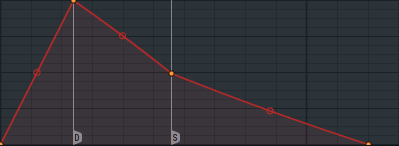
\includegraphics[width=.95\linewidth]{images/ADSR.png}
	\caption{ADSR}
	\label{ADSR}
\end{figure}


\begin{tabularx}{\textwidth}{|l|X|X|X|X|X|}
	\hline
	Wert & Attack (Sek.) & Decay (Sek.)  & Sustain (Verhältnis) & Release (Sek.) Wert $\leq$ F & Release (Sek.) Wert $>$ F \\
	\hline
	00 & 4.1 & 1.2 (\$ED) & 1/8 & Unendlich & 1.2\\
	\hline
	01 & 2.6 & 0.74 (\$ED) & 1/8 & 38 & 0.88 \\
	\hline
	02 & 1.5 & 0.44 (\$ED) & 2/8 & 28 & 0.74 \\
	\hline
	03 & 1.0 & 0.29 (\$ED) & 2/8 & 24 & 0.59 \\
	\hline
	04 & 0.64 & 0.18 (\$ED) & 3/8 & 19 & 0.44 \\
	\hline
	05 & 0.38 & 0.11 (\$ED) & 3/8 & 14 & 0.37 \\
	\hline
	06 & 0.26 & 0.074 (\$ED) & 4/8 & 12 & 0.29 \\
	\hline
	07 & 0.16 & 0.037 (\$ED) & 4/8 & 9.4 & 0.22 \\
	\hline
	08 & 0.096 & 1.2 & 5/8 & 7.1 & 0.18 \\
	\hline
	09 & 0.064 & 0.74 & 5/8 & 5.9 & 0.15 \\
	\hline
	0A & 0.04 & 0.44 & 6/8 & 4.7 & 0.11 \\
	\hline
	0B & 0.024 & 0.29 & 6/8 & 3.5 & 0.092 \\
	\hline
	0C & 0.016 & 0.18 & 7/8 & 2.9 & 0.074 \\
	\hline
	0D & 0.01 & 0.11 & 7/8 & 2.4 & 0.055 \\
	\hline
	0E & 0.006 & 0.074 & 1 & 1.8 & 0.037 \\
	\hline
	0F & 0 & 0.037 & 1 & 1.5 & 0.018 \\
	\hline
\end{tabularx}

\bigskip

Die Tabelle und die beiden unterschiedlichen Befehle zur ADSR Beschreibung benötigen eine genauere Erklärung. Diese erfolgt am Beispiel unseres Custom Instruments.


\medskip

\lstinputlisting[framexleftmargin=8mm, frame=shadowbox, rulesepcolor=\color{blue}, numbers=left, firstline=1, lastline=5]{codes/ADSR.txt}

\medskip

Beide Befehle beschreiben die gleichen ADSR Werte. Als erstes sei gesagt, dass die Reihenfolge der ADSR Werte nicht \$AD \$SR, sondern \$DA \$SR entspricht. \\
Als nächstes fällt auf, dass sich der Decay Wert unterscheidet. Der Decay Wert in \#instruments\{\} muss immer um 8 aufaddiert werden. \\
Sustain und Release Werte hängen voneinander ab. In diesem Beispiel ist die Release Dauer nicht unendlich, obwohl der Release Wert auf 0 steht. Für eine Release Dauer von unendlich muss der Sustain Wert immer eine gerade Zahl sein. Hier müsste der Sustain Wert auf A gesetzt werden, damit das Sustain Verhältnis gleich bleibt, die Release Dauer aber unendlich beträgt. \\
Falls \$DA in \#instruments\{\} kleiner als \$80 ist, wird automatisch Gain aktiviert. Genauso wird Gain aktiviert, falls im \$ED Befehl der \$DA Wert $\geq 80$ ist.

\bigskip

Das Instrument wird durch ADSR wie folgt beschrieben: \\
\textbf{Attack:} 0 Sek. \\
\textbf{Decay:} 0.29 Sek. \\
\textbf{Sustain:} 6/8 vom Maximum \\
\textbf{Release:} 1.2 Sek.



\subsubsection{Gain}

Neben ADSR kann ein Instrument auch durch Gain beschrieben werden. Wie bei ADSR gibt es zwei Möglichkeiten, Gain zu definieren. Zum einen durch das dritte Argument in \#instruments\{\} (wird dort aber nur aktiv, falls \$DA in \#instruments\{\} kleiner als \$80 ist), zum anderen durch die Hexbefehle \$FA \$01 \$XX oder \$ED \$80+ \$XX. \\
Gain beschreibt keine vollständige Hüllkurve sondern nur das Anschlag- oder Abklingverhalten eines Instruments. Im Vergleich zu ADSR bietet Gain allerdings auch exponentielle Verläufe an, wohingegen durch ADSR nur lineare Verläufe möglich sind. \\
Es gibt fünf verschiedene Gain Modi:

\medskip

\begin{itemize}
	\item \textbf{Direct}
	\item \textbf{Decrease}
	\item \textbf{Exponential Decrease}
	\item \textbf{Increase}
	\item \textbf{Bent Line Increase}
\end{itemize}


\bigskip

Bei Gain Werten zwischen 00 bis 7F ist der Modus Direct aktiv (direkter Anschlag).
Die weiteren Modi inklusive Anstiegs- und Abklingszeiten stehen in der folgenden Tabelle:

\bigskip

\begin{table}[htbp]
\begin{tabularx}{\textwidth}{|X|X|}
	\hline
	Zeit von Wert 7F bis 0: & Zeit von Wert 0 bis 7F: \\
	\hline
\end{tabularx}

\begin{tabularx}{\textwidth}{|l|X|l|X|l|X|l|X|}
	\hline
	Wert & Decrease & Wert & Exp Decrease & Wert & Increase & Wert & Bent Line Increase \\
	\hline
	80 & Unendlich & A0 & Unendlich & C0 & Unendlich & E0 & Unendlich \\
	\hline
	81 & 4.1 s & A1 & 38 s & C1 & 4.1 s & E0 & 7.2 s \\
	\hline
	82 & 3.1 s & A2 & 28 s & C2 & 3.1 s & E2 & 5.4 s \\
	\hline
	83 & 2.6 s & A3 & 24 s & C3 & 2.6 s & E3 & 4.6 s \\
	\hline
	84 & 2.0 s & A4 & 19 s & C4 & 2.0 s & E4 & 3.5 s \\
	\hline
	85 & 1.5 s & A5 & 14 s & C5 & 1.5 s & E5 & 2.6 s \\
	\hline
	86 & 1.3 s & A6 & 12 s & C6 & 1.3 s & E6 & 2.3 s \\
	\hline
	87 & 1.0 s & A7 & 9.4 s & C7 & 1.0 s & E7 & 1.8 s \\
	\hline
	88 & 770 ms & A8 & 7.1 s & C8 & 770 ms & E8 & 1.3 s \\
	\hline
	89 & 640 ms & A9 & 5.9 s & C9 & 640 ms & E9 & 1.1 s \\
	\hline
	8A & 510 ms & AA & 4.7 s & CA & 510 ms & EA & 900 ms \\
	\hline
	8B & 380 ms & AB & 3.5 s & CB & 380 ms & EB & 670 ms \\
	\hline
	8C & 320 ms & AC & 2.9 s & CC & 320 ms & EC & 560 ms \\
	\hline
	8D & 260 ms & AD & 2.4 s & CD & 260 ms & ED & 450 ms \\
	\hline
	8E & 190 ms & AE & 1.8 s & CE & 190 ms & EE & 340 ms \\
	\hline
	8F & 160 ms & AF & 1.5 s & CF & 160 ms & EF & 280 ms \\
	\hline
	90 & 130 ms & B0 & 1.2 s & D0 & 130 ms & F0 & 220 ms \\
	\hline
	91 & 96 ms & B1 & 880 ms & D1 & 96 ms & F1 & 170 ms \\
	\hline
	92 & 80 ms & B2 & 740 ms & D2 & 80 ms & F2 & 140 ms \\
	\hline
	93 & 64 ms & B3 & 590 ms & D3 & 64 ms & F3 & 110 ms \\
	\hline
	94 & 48 ms & B4 & 440 ms & D4 & 48 ms & F4 & 84 ms \\
	\hline
	95 & 40 ms & B5 & 370 ms & D5 & 40 ms & F5 & 70 ms \\
	\hline
	96 & 32 ms & B6 & 290 ms & D6 & 32 ms & F6 & 56 ms \\
	\hline
	97 & 24 ms & B7 & 220 ms & D7 & 24 ms & F7 & 42 ms \\
	\hline
	98 & 20 ms & B8 & 180 ms & D8 & 20 ms & F8 & 35 ms \\
	\hline
	99 & 16 ms & B9 & 150 ms & D9 & 16 ms & F9 & 28 ms \\
	\hline
	9A & 12 ms & BA & 110 ms & DA & 12 ms & FA & 21 ms \\
	\hline
	9B & 10 ms & BB & 92 ms & DB & 10 ms & FB & 18 ms \\
	\hline
	9C & 8 ms & BC & 74 ms & DC & 8 ms & FC & 14 ms \\
	\hline
	9D & 6 ms & BD & 55 ms & DD & 6 ms & FD & 11 ms \\
	\hline
	9E & 4 ms & BE & 37 ms & DE & 4 ms & FE & 7 ms \\
	\hline
	9F & 2 ms & BF & 18 ms & DF & 2 ms & FF & 3.5 ms \\
	\hline
\end{tabularx}
\caption{Gain Table von ggamer77}
\end{table}

\medskip

Decrease und Exponential Decrease werden nur wirksam, wenn sie während einer gespielten Note aktiviert wird. Dies können wir mittels Haltebogen erreichen.

\bigskip

Im SPC700 Player werden die einzelnen Modi wie folgt angezeigt: 

\bigskip

\begin{tabularx}{\textwidth}{l l}
Direct & 
\textcolor{blue}{Ga}
\textcolor{red}{D}
- -
\\
Decrease & 
\textcolor{blue}{Ga}
\textcolor{green}{A}
0 0
\\
Exponential Decrease & 
\textcolor{blue}{Ga}
\textcolor{green}{A}
0
\textcolor{red}{1}
\\
Increase &
\textcolor{blue}{Ga}
\textcolor{green}{A}
\textcolor{red}{1}
0
\\
Bent Line Increase &
\textcolor{blue}{Ga}
\textcolor{green}{A}
\textcolor{red}{1}
\textcolor{red}{1}
\end{tabularx}

\bigskip

Die geänderten ADSR Werte durch \$ED bzw. Gain Wert durch \$FA \$01 oder \$ED werden mit erneutem Aufrufen des Instruments (@) wieder zurückgesetzt.

\subsection{Sample Groups}

Wer bereits häufiger Musik in eine Rom gepatcht oder sampled Songs selbst geschrieben hat, wird wahrscheinlich schon auf Sample Groups gestoßen sein. \\
Sample Groups sind -- wie der Name schon vermuten lässt -- eine vordefinierte Gruppe an Samples. AddMusicK stellt die Sample Groups \#default und \#optimized zur Verfügung. Diese beinhalten alle SMW Samples, die für Local Songs (normale Hintergrundmusik), Global Songs (Hintergrundmusik, die in allen Leveln geladen sind, z.B. Stage Clear oder P-Block) und Soundeffekte verwendet werden.
Sie befinden sich in \textit{samples/default/} bzw. \textit{samples/optimized/}.

\bigskip

Sofern kein \#samples\{\} Block verwendet wird, setzt AddMusicK versteckt die Sample Group \#default. Sobald \#samples\{\} benutzt wird, muss eine Sample Group gesetzt werden.
Ohne Sample Group wird nur das Standardinstrument @0 geladen, alle anderen SMW Samples können dann nicht mehr verwendet werden. \\
In eine Rom gepatcht hat dies außerdem zur Folge, dass weder Global Songs noch Soundeffekte richtig abgespielt werden. Das liegt daran, dass jeder Soundeffekt in SMW aus den gleichen Samples erzeugt werden, die auch für die Musikinstrumente benutzt werden.
Stattdessen werden Custom Samples die im \#samples\{\} Block liegen verwendet. Sobald ein sampled Song geschrieben wird, muss also eine Sample Group gesetzt werden.

\bigskip

Bei der Sample Group \#default handelt es sich um die original SMW Samples, die Samples aus \#optimized beinhalten nur die Hälfte der Informationen, wodurch diese auch nur halb so groß sind.
Der Informationsverlust bedeutet eine geringere Soundqualität, diese ist aber kaum wahrnehmbar. Die Wahl der Sample Group hängt also nur davon ab, wie viel freier Speicher noch im Arbeitsspeicher vorhanden ist.

\subsubsection*{Custom Sample Groups}

Es ist auch möglich eine eigene Sample Group anzulegen. Hauptmotivation ist, etwas Arbeitsspeicher einzusparen, indem einzelne Samples aus der Sample Group durch die Datei \textit{EMPTY.brr} ersetzt werden. Dabei handelt es sich um ein Sample ohne Informationen und dient nur als Platzhalter, damit alle anderen Samples ihre richtige Position in der Liste beibehalten.

\bigskip

In \textit{Addmusic\_sample groups.txt} werden alle Sample Groups definiert. Zwei Dinge fallen auf: Zum einen scheint es, als würden Samples fehlen. Die Samples @11, @16, @18, @23 - @28 werden jedoch nur durch die Samples aus der Liste erzeugt, die aber andere ADSR Einstellungen besitzen. \\

Zum anderen stehen hinter den Samples @14, @17 und @21 keine Ausrufezeichen. Ein Ausrufezeichen hinter einem Samplenamen bewirkt, dass diese global (also dauerhaft) geladen sind, solange die Sample Group verwendet wird. Die Samples @14, @17 und @21 sind die einzigen Samples, die weder für Global Songs, noch Soundeffekte und ausschließlich für einige Local Songs verwendet werden und daher nicht global geladen werden müssen. \\
Unter \href{https://www.smwcentral.net/?p=viewthread\&t=97787}{https://www.smwcentral.net/?p=viewthread\&t=97787} ist eine vollständige Liste, welche Samples für welche Soundeffekte und Global Songs verwendet werden. \\
Die populärsten Samples die durch \textit{EMPTY.brr} ersetzt werden sind \textit{12 SMW @15.brr} (wird nur für Yoshi Sound verwendet), \textit{09 SMW @7.brr} (wird nur für den Global Song Bonus End verwendet) und \textit{13 SMW Thunder.brr}. Eine Sample Group ohne \textit{12 SMW @15.brr} wäre daher nicht kompatibel mit Leveln, die Yoshi benutzen. Daher muss immer darauf hingewiesen werden, welche Sounds oder Global Songs nicht mehr funktionieren, wenn man einen Song teilt oder hochlädt.

\bigskip

Falls eine neue Sample Group angelegt werden soll, kopiert man dafür am einfachsten die Sample Group \#optimized aus \textit{Addmusic\_sample groups.txt}, fügt diese im Textdokument ein mit einem anderen Namen als optimized und ersetzt Samples, die nicht verwendet werden sollen durch \textit{\dq EMPTY.brr\dq{}!}. Im Song selbst wird die Sample Group schließlich mit \#SampleGroupName geladen.

\subsection{Eigene Samples erstellen}


Jede Audioquelle, die sich in eine .wav Datei konvertieren lässt, sind potentielle Samples die sich in Songs benutzen lassen. Als erstes öffnen wir Audacity und laden unsere Sounddatei ein
(z.B. .mp3 oder .wav). Mit dem Selection Tool (\textit{F1}) markieren wir nun alle Bereiche, die entfernt werden sollen und löschen diese mit \textit{Entf}. Danach klicken wir links auf den kleinen Pfeil neben dem Dateinahmen und wählen dort \textit{Split Stereo to Mono} aus.

\begin{figure}[htbp] \centering
	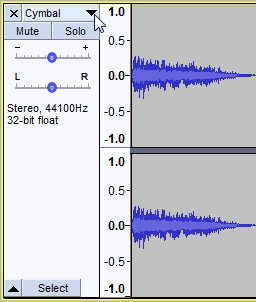
\includegraphics[width=.50\linewidth]{images/Audacity.png}
	\caption{Track aufteilen in Audacity}
	\label{Audacity}
\end{figure}

\bigskip

Dadurch beugen wir vor, dass das Sample im nächsten Schritt nicht nur auf einem Lautsprecher zu hören ist. Außerdem wird dadurch die Größe des Samples ungefähr halbiert. \\
Es ist auch möglich, 2 Stereo Samples zu erzeugen. Dafür muss \textit{Split Stereo Track} anstatt \textit{Split Stereo to Mono} ausgewählt werden. Das hat allerdings den Nachteil, dass 2 Samples für einen Sound benötigt werden, was wiederum bedeutet, dass doppelt so viel Speicher verbraucht wird und im Song selbst 2 Kanäle belegt werden müssen.

\bigskip

Die Datei wird nun als .wav Datei exportiert mit einer Signed 16-bit PCM Codierung.

\bigskip

Als nächstes öffnen wir OpenMTP, laden unsere exportierte .wav ein und klicken oben auf den Reiter \textit{Samples}. Es öffnet sich folgendes Fenster:

\begin{figure}[htbp] \centering
	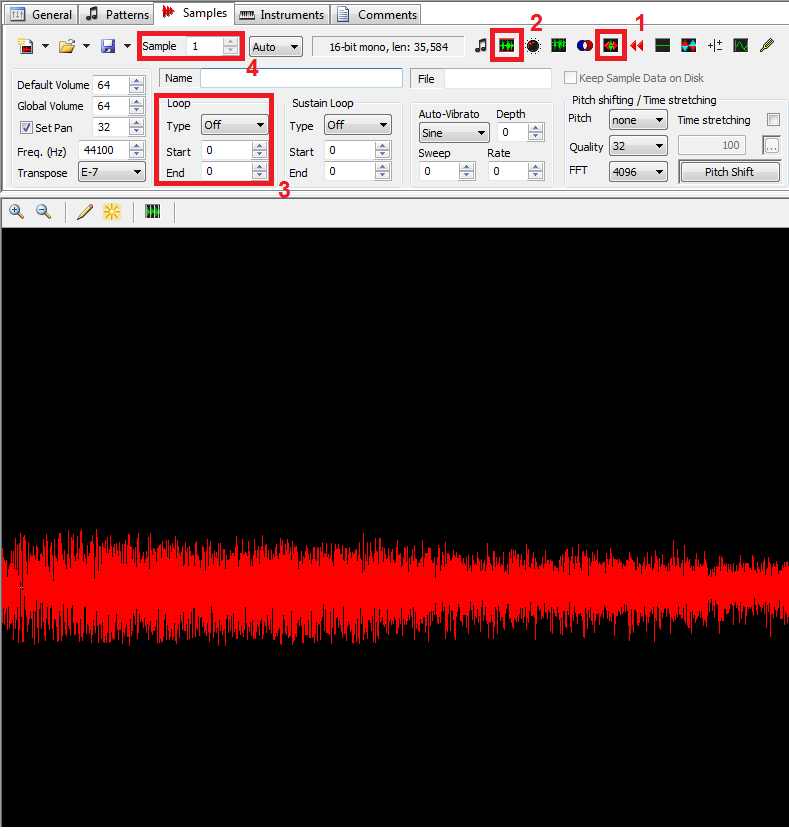
\includegraphics[width=.95\linewidth]{images/OpenMTP.png}
	\caption{Samples bearbeiten in OpenMTP}
	\label{OpenMTP}
\end{figure}

\bigskip

Wir benötigen nur die 4 markierten Funktionen. Diese sind:

\medskip

\begin{itemize}
	\item \textbf{1. Up-/Down Sampling}
	\item \textbf{2. Normalize}
	\item \textbf{3. Loop Points}
	\item \textbf{4. Sample Auswahl} 
\end{itemize}

\medskip

Punkt 1 benutzen wir zum Downsamplen. Damit ist gemeint, dass die Samplerate -- also die Abtastrate -- verringert wird. Voreingestellt ist eine Samplerate von 44.1 kHz, halbieren wir diese durch downsamplen auf 22.05 kHz wird unser Signal nur noch mit der halben Anzahl an Samples (damit sind die Abtastpunkte gemeint) abgetastet. Die Konsequenzen sind, dass die Hälfte an Informationen gelöscht werden, was in ein halb so großes Signal mit Qualitätsverlust resultiert. Außerdem wird die akustisch wahrnehmbare Frequenz bei gleichem Pitch verdoppelt was wir an anderer Stelle ausnutzen können. \\
In der Regel sollte man ein- bis maximal zweimal downsamplen um das Sample klein genug zu bekommen.

\bigskip

Punkt 2 verstärkt unser gesamtes Sample im gleichen Maß ohne Clipping zu erzeugen (Abschneiden der Amplitude). Es ist immer einfacher, ein Sample im nachhinein leiser einzustellen als lauter, weshalb wir diese Option immer benutzen sollten.

\bigskip

Punkt 3 benötigen wir nur für Samples die loopen, also unendlich lang zu hören sind, solange eine Note nicht aufhört zu spielen.  Dieser Punkt ist recht anspruchsvoll, da es nicht einfach ist, Start und Endpunkte zu finden, die ein Sample sauber loopen zu lassen. Besonders bei stark heruntergesampleten Signalen fängt ein Sample schnell an zu \dq schwingen\dq{}. \\
Wichtig hierbei ist, dass beide Looppunkte ein vielfaches von 16 sein müssen, falls wir im nächsten Schritt split700 benutzen sollten. Wird stattdessen das C700 VST Plugin verwendet, korrigiert dieses automatisch unsere in OpenMTP gesetzten Looppunkte. \\
Sustain Loop benötigen wir nicht. Dieses beschreibt einen Loop der verlassen wird, sobald das Sample nicht mehr gespielt wird und dadurch das Ende zu hören ist. Da es kein echtes Release Event in AddMusicK gibt und ein Sample mit Ende einer Note sofort aufhört zu spielen, kann in einem geloopten Sample der Rest des Signals hinter dem End Loop Punkt gelöscht werden, weil dieses nie erreicht wird.


\bigskip

Punkt 4 wird nur benötigt, falls wir vorher in Audacity das Sample auf 2 Stereo Tracks aufgeteilt haben. Hier kann zwischen den einzelnen Samples hin und her gewechselt werden.

\bigskip

Ist das Sample fertig bearbeitet, kann es über das Diskettensymbol neben Punkt 4 wieder als .wav Datei gespeichert werden. \\
Als letzten Schritt muss die .wav Datei nur noch in eine .brr Datei konvertiert werden. Dafür benutzen wir entweder das C700 Plugin (bevorzugt) oder split700.

%Der allgemeine Konvertierungsprozess wie hier beschrieben stammt größtenteils von Wakana mit Ausnahmen einiger technischer Erklärungen.
\section{Ticks, Song Stats und Hexbefehle}

Dieses Kapitel beschäftigt sich rund um das Thema Hexwerte und Hexbefehle. Es werden die meisten, aber nicht alle Hexbefehle vorgestellt, es handelt sich hierbei jedoch um die wichtigsten. \\
Unter \textit{AddmusicK/readme\_files/hex\_command\_reference.html} befindet sich eine vollständige Liste aller Hexbefehle.

\subsection*{Einschub: Hexadezimalsystem}

Das Hexadezimalsystem ist ein Zahlensystem mit Basis 16. Dabei sind die ersten 16 Ziffern (von 0 bis 15) folgende:
0, 1, 2, 3, 4, 5, 6, 7, 8, 9, A, B, C, D, E, F \\

Um eine Hexzahl von einer Dezimalzahl zu unterscheiden, kommen diese mit Präfixen daher, wie z.B. 0x oder \$. So weiß man, dass es sich bei 0x12 (gesprochen Eins Zwei) um eine 18 im Dezimalsystem und nicht eine Zwölf handelt. Mit dem Windows Taschenrechner auf Programmierer eingestellt lässt sich zudem zwischen verschiedenen Zahlensystemen bequem umrechnen.


\subsection{Ticks}

Songs die wir mit AddMusicK schreiben sind in Notenwerten, Pausen und Events zeitlich quantisiert.
Die Auflösung beträgt 48 PPQ (pulses per quarter note, deutsch Impulse pro Viertelnote) bzw. 48 TPQN (ticks per quarter note, deutsch Ticks pro Viertelnote). In FL Studio kann der PPQ Wert unter \textit{Options/Project General Settings} eingestellt werden.\\
Der kleinste zeitliche Schritt -- unabhängig vom Tempo -- ist 1 Tick. Dieser hat die Länge einer 192stel Note. Zwischen klassischen Notenwerten und Tick Werten kann also über das Verhältnis 192/Notenwert umgerechnet werden. Anstatt einem Notenwert hinter einer Note oder Pause kann mit einem Gleichheitszeichen = ein Tick Wert angegeben werden. Beispiel:

\bigskip

c2 $ \equiv $ c=96 (Rechnung: $ \dfrac{192}{c2} $)\\
r4\textasciicircum16 $ \equiv $ r=60 (Rechnung: $ \dfrac{192}{r4} +  \dfrac{192}{r16} $)\\

\bigskip

Die Auflösung von 48 PPQ hat zwei Dinge zur Folge: Unsere kleinste Note ist eine 192stel Note, eine 256stel Note ist daher nicht möglich darzustellen. Außerdem wird beispielsweise eine 128stel Note nicht richtig aufgelöst, da diese bei 48 PPQ 1.5 Ticks lang ist $(\dfrac{192}{128} = 1.5$). Stattdessen wir eine 128stel Note auf 1 Tick abgeschnitten, was wiederum einer 192stel Note entspricht. \\
Tick Werte treffen wir oft in Dateien an, die mit einem SPC/MML Konverter konvertiert wurden. Für extrem kurze Noten, beispielsweise um einen Swing Rhytmus zu erzeugen, können Tick Werte intuitiver sein als die klassischen Notenwerte.

\bigskip

Am häufigsten jedoch benutzen wir Tick Werte in Hexbefehlen. Sobald eine Dauer für einen Hexbefehl angeben wird, ist diese ein Tick Wert als Hexzahl ausgedrückt. Am Beispiel unseres Panning Befehls aus Kapitel \ref{sec:ErstenSongSchreiben} sehen wir, dass bei \$DC \$C0 \$05 die Länge \$C0 als Dezimalzahl 192 entspricht, was als Tick Wert wiederum eine ganzen Note ist. \\
Alternativ befindet sich im Anhang eine Tabelle mit einigen Längen die als Hexwerte dargestellt sind.

\subsection{Stats}

Sobald wir einen Song mit AddMusicK porten, wird automatisch im Verzeichnis \textit{AddMusicK/Stats/} ein gleichnamiges Textdokument mit verschiedenen Statistiken angelegt.

\bigskip

\begin{figure}[htbp] \centering
	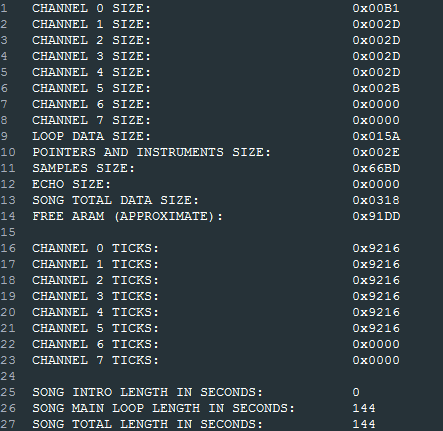
\includegraphics[width=.80\linewidth]{images/stats.png}
	\caption{Statistiken eines Songs}
	\label{stats}
\end{figure}

Channel Size 0 bis 7 geben die allgemeine Größe in Bytes als Hexwert dargestellt an,
Loop Data Size, wie viel Speicher durch das definieren der Loops selbst und deren Inhalte verbraucht wird und Pointers and Instruments Size von Pointern und Instrumentendefinitionen. \\
Die Summe dieser Werte ergibt die Total Data Size (auch Insert Size genannt) die beispielsweise angegeben werden muss, wenn ein Song auf SMW Central hochgeladen werden soll. \\
Samples Size gibt die Größe aller eingebundenen Samples und der Samples aus der Sample Group an, Echo Size von Echo, falls man diesen aktiviert.

\bigskip

Wird die Summe aus Insert Size, Samples Size und Echo Size von 64kB abgezogen (die Menge an Arbeitsspeicher vom SPC700) erhalten wir den Free ARAM (approximate) Wert, also jener Wert, der den freien Speicher im Audio Ram angibt. \\
Von diesem Wert müssen wir aber ungefähr 0x2700 Bytes abziehen (ca. 10kB), sofern keine Global Songs oder Sample Groups geändert wurden. Dieser Platz wird von der Musik Engine, Soundeffekten und Global Songs dauerhaft eingenommen und wird nicht in der Rechnung im Stats Textdokument berücksichtigt. Wird beispielsweise ein Global Song ausgetauscht, ändert sich die Grenze entsprechend.

\bigskip

Channel Ticks 0 - 7 geben die Länge der Kanäle in Ticks an, wobei es sich hierbei um Dezimalzahlen und nicht um Hexwerte handelt, trotz des fälschlicherweise verwendeten Präfixes. Im Idealfall besitzen alle verwendeten Kanäle die gleiche Länge, da der kürzeste Kanal die Gesamtdauer des Songs angibt.

\bigskip

Die letzten 3 Werte geben die Länge des Intros, des geloopten Song selbst und der Summe aus Intro und geloopten Song in Sekunden an.

\subsection{Hexbefehle}

Hexbefehle sind einfach durch ihren Aufbau zu identifizieren. Sie beginnen mit einem \$ und einer Befehlsnummer als Hexadezimalzahl, gefolgt von ein bis maximal 3 Hexwerten (einzige Ausnahme sind die Filter Koeffizienten).
\bigskip

Falls ein Befehl eine Länge oder Dauer als Parameter verwendet, handelt es sich hierbei immer um einen Tick Wert im Hexadezimalsystem. Eine Tabelle für einige Standardlängen findet sich im Anhang in Tabelle \ref{tickshex}.

\subsubsection{Pan Fading}

Pan Fading beschreibt den Verlauf der Lautstärke eines Instruments zwischen den Lautsprechern.

\medskip

\lstinputlisting[framexleftmargin=8mm, frame=shadowbox, rulesepcolor=\color{blue}, numbers=left, firstline=2, lastline=2]{codes/Hex.txt}

\medskip

mit 

\begin{itemize}
	\item Dauer \$XX 
	\item Ziel Panning \$YY
\end{itemize}

wobei \$00 y0 (Lautstärke vollständig rechts), \$0A y10 (Lautstärke gleichmäßig verteilt) und \$14 y20 (Lautstärke vollständig links) entspricht.

\subsubsection{Tempo Fading}

Tempo Fading beschreibt den globalen Verlauf des Tempos.

\medskip

\lstinputlisting[framexleftmargin=8mm, frame=shadowbox, rulesepcolor=\color{blue}, numbers=left, firstline=4, lastline=4]{codes/Hex.txt}

\medskip

mit 

\begin{itemize}
	\item Dauer \$XX 
	\item Ziel Panning \$YY
\end{itemize}

Dabei kann sich der Befehl in einem beliebigen Kanal befinden.

\subsubsection{Global volume Fading}

Global Volume Fading beschreibt den Verlauf der globalen Lautstärke.

\medskip

\lstinputlisting[framexleftmargin=8mm, frame=shadowbox, rulesepcolor=\color{blue}, numbers=left, firstline=6, lastline=6]{codes/Hex.txt}

\medskip

mit

\begin{itemize}
	\item Dauer \$XX 
	\item Ziel Lautstärke \$YY
\end{itemize}

Dabei kann sich der Befehl in einem beliebigen Kanal befinden.

\subsubsection{Vol Fading}

Volume Fading beschreibt den Verlauf der Lautstärke eines einzelnen Kanals.

\medskip

\lstinputlisting[framexleftmargin=8mm, frame=shadowbox, rulesepcolor=\color{blue}, numbers=left, firstline=8, lastline=8]{codes/Hex.txt}

\medskip

mit 

\begin{itemize}
	\item Dauer \$XX
	\item Ziel Lautstärke \$YY 
\end{itemize}

\subsubsection{Pitch Bending}

Pitch Bending schreibt den Verlauf des Pitches einer Note. Prominentes Beispiel dafür ist eine Gitarrensaite, die man nach oben oder unten schiebt.

\medskip

\lstinputlisting[framexleftmargin=8mm, frame=shadowbox, rulesepcolor=\color{blue}, numbers=left, firstline=10, lastline=10]{codes/Hex.txt}

\medskip

mit

\begin{itemize}
	\item Verzögerung \$XX
	\item Dauer \$YY
	\item Ziel Note \$ZZ
\end{itemize}

Der Befehl steht hinter der Note, die ein Pitch Bending erfahren soll. \\
Die Verzögerung gibt an, wann der Befehl ausgeführt werden soll, die Dauer gibt an wie lange das Bending dauert. Der Hexwert \$ZZ, der eine Note beschreibt, ist in Tabelle \ref{Noten} nachzulesen.

\begin{table}
\begin{tabularx}{\textwidth}{|l|X|X|X|X|X|X|X|X|X|X|X|X|}
	\hline
	& C & C\# & D & D\# & E & F & F\# & G & G\# & A & A\# & B   \\
	\hline
	o1 & 80 & 81 & 82 & 83 & 84 & 85 & 86 & 87 & 88 & 89 & 8A & 8B \\
	\hline
	02 & 8C & 8D & 8E & 8F & 90 & 91 & 92 & 93 & 94 & 95 & 96 & 97 \\
	\hline
	o3 & 98 & 99 & 9A & 9B & 9C & 9D & 9E & 9F & A0 & A1 & A2 & A3 \\
	\hline
	o4 & A4 & A5 & A6 & A7 & A8 & A9 & AA & AB & AC & AD & AE & AF \\
	\hline
	o5 & B0 & B1 & B2 & B3 & B4 & B5 & B6 & B7 & B8 & B9 & BA & BB \\
	\hline
	o6 & BC & BD & BE & BF & C0 & C1 & C2 & C3 & C4 & C5 & & \\
	\hline
\end{tabularx}
\caption{Noten als Hexwerte}
\label{Noten}
\end{table}


Es gibt zudem Wege, den Befehl einfacher auszuführen.

\bigskip

Anstelle des \$ZZ Wertes kann auch direkt eine Note angegeben werden (inklusive Oktavwechsel). Wichtigster Unterschied ist, dass durch ein Pitch Bending mit \$ZZ kein Oktavwechsel für nachfolgende Noten statt findet. Beispiel:

\medskip

\lstinputlisting[framexleftmargin=8mm, frame=shadowbox, rulesepcolor=\color{blue}, numbers=left, firstline=11, lastline=12]{codes/Hex.txt}

\medskip

Beide Befehle führen ein Pitch Bending von o3f nach o4c durch, allerdings ist die nachfolgende Note im ersten Befehl ein o3e und im zweiten ein o4e.

\bigskip

Zusätzlich kann durch den Einsatz von Haltebögen ein Hexbefehl anschaulicher beschrieben werden, in einigen Fällen sind diese auch notwendig um innerhalb einer Note mehrere oder unterschiedliche Befehle auszuführen. Beispiel:

\medskip

\lstinputlisting[framexleftmargin=8mm, frame=shadowbox, rulesepcolor=\color{blue}, numbers=left, firstline=13, lastline=14]{codes/Hex.txt}

\medskip

Beide Befehle beschreiben den gleichen Vorgang. Der erste Befehl wird erst nach der Verzögerungszeit von \$30 Ticks (entspricht der Länge einer Viertelpause) ausgeführt. Der zweite Befehl spielt die c+4 Note, ohne den Pitch Bending Befehl zu benutzen, der Befehl wird dann aber auf den Teil des Haltebogens sofort angewendet. Dieses Beispiel verdeutlicht auch, dass Vorsicht geboten ist bei Noten mit Haltebögen, die mit Pitch Bendings bearbeitet werden sollen.

\bigskip

Außerdem muss darauf geachtet werden, Haltebögen bei Noten mit Notenlängen größer 2 richtig anzuwenden. AddMusicK interpretiert diese intern auch mit Haltebögen. Ein c1 wird von AddMusicK beispielsweise als ein c2\textasciicircum2 gehandhabt. Dadurch entstehen Fehler. Beispiel:

\medskip

\lstinputlisting[framexleftmargin=8mm, frame=shadowbox, rulesepcolor=\color{blue}, numbers=left, firstline=15, lastline=16]{codes/Hex.txt}

\medskip

Zeile 2 zeigt, wie der Befehl der ersten Zeile von AddMusicK interpretiert wird. Das Pitch Bending würde nie ausgeführt werden, da eine halbe Note lang nichts passiert und danach eine weitere halbe Note lang (\$60) Verzögert wird, bis der Befehl ausgeführt werden soll. Es wird also eine ganze Note lang gewartet, bevor überhaupt das Bending beginnen würde.

Soll c1 nach einer halben Note das Pitch Bending beginnen, muss der Befehl wie folgt umgeschrieben werden:

\medskip

\lstinputlisting[framexleftmargin=8mm, frame=shadowbox, rulesepcolor=\color{blue}, numbers=left, firstline=17, lastline=17]{codes/Hex.txt}

\medskip



\subsubsection{Vibrato}

Vibrato beschreibt das Schwingen um eine Tonhöhe.

\medskip

\lstinputlisting[framexleftmargin=8mm, frame=shadowbox, rulesepcolor=\color{blue}, numbers=left, firstline=19, lastline=19]{codes/Hex.txt}

\medskip

mit

\begin{itemize}
	\item Verzögerung \$XX
	\item Frequenz  \$YY, wie schnell geschwungen wird
	\item Amplitude \$ZZ, mit der um eine Note geschwungen wird
\end{itemize}

Der Befehl wird auf alle nachfolgenden Noten des Kanals angewendet. \\
Mit \$DF kann das Vibrato ausgeschaltet werden. \\
Zusätzlich kann Vibrato Fading eingestellt werden:

\medskip

\lstinputlisting[framexleftmargin=8mm, frame=shadowbox, rulesepcolor=\color{blue}, numbers=left, firstline=20, lastline=20]{codes/Hex.txt}

\medskip

mit

\begin{itemize}
	\item Dauer \$XX
\end{itemize}

Dabei muss Vibrato Fading immer nach Vibrato benutzt werden, da sich der \$EA Befehl auf die \$YY und \$ZZ Werte von \$DE bezieht. Beispiel:

\medskip

\lstinputlisting[framexleftmargin=8mm, frame=shadowbox, rulesepcolor=\color{blue}, numbers=left, firstline=21, lastline=22]{codes/Hex.txt}

\medskip

Die erste Zeile beschreibt ein c1, dass nach der Dauer einer halben Note anfängt zu schwingen.
Die zweite Zeile beschreibt ein c1, dass nach der Dauer einer halben Note anfängt, anzuschwingen,
und erreicht das vorher definierte Vibrato Verhalten nach einer Viertelnote.


\subsubsection{ADSR / Gain einstellen}

ADSR kann während der Laufzeit verändert werden.

\medskip

\lstinputlisting[framexleftmargin=8mm, frame=shadowbox, rulesepcolor=\color{blue}, numbers=left, firstline=24, lastline=24]{codes/Hex.txt}

\medskip

wobei der Da Wert zwischen \$00 und \$7F liegen muss, ansonsten wird Gain aktiviert.

\bigskip

Genauso kann Gain umgestellt werden.

\medskip

\lstinputlisting[framexleftmargin=8mm, frame=shadowbox, rulesepcolor=\color{blue}, numbers=left, firstline=25, lastline=25]{codes/Hex.txt}

\medskip

mit \$YY dem Gain Wert. \$80 kann auch größer sein, darf aber nicht kleiner sein, ansonsten wird ADSR aktiviert. \\

Wird ein Instrument mit @ aufgerufen, werden die ADSR bzw. Gain Werte, die durch \$ED eingestellt wurden, zurückgesetzt. \\
Weitere Informationen zu ADSR und Gain siehe Kapitel \ref{sec:ADSR} und \ref{sec:Gain}.

\subsubsection{Echo}

Mit Echo kann der Raumklang eingestellt werden.

\medskip

\lstinputlisting[framexleftmargin=8mm, frame=shadowbox, rulesepcolor=\color{blue}, numbers=left, firstline=27, lastline=27]{codes/Hex.txt}

\medskip

mit

\begin{itemize}
	\item Kanäle \$XX
	\item Echo Lautstärke links \$YY
	\item Echo Lautstärke rechts \$ZZ
\end{itemize}

Welche Kanäle Echo erfahren sollen, wird mit \$XX festgelegt. Diese werden Bitweise durch die Kanäle in umgekehrter Reihenfolge bestimmt und letztendlich als Hexwert dargestellt. Ein Beispiel:

\bigskip

Die Kanäle 5, 6 und 7 (\#4, \#5 und \#6) sollen Echo erhalten. Wir schreiben die Kanalnummern absteigend auf und setzen eine 1 für Echo, ansonsten 0.

\begin{table}[htbp]
	\centering
	\begin{tabularx}{8.5cm}{|X|c|c|c|c|c|c|c|c|}
		\hline
		Kanalnummer: & 7 & 6 & 5 & 4 & 3 & 2 & 1 & 0 \\
		\hline
		Bits: & 0 & 1 & 1 & 1 & 0 & 0 & 0 & 0 \\
		\hline
	\end{tabularx}
\end{table}


Wir erhalten die Binärzahl 0b1110000 (0b ist der Präfix für Binärzahlen). Als Hexadezimalzahl ist dies \$70.

\bigskip

Zusätzlich müssen weitere Parameter eingestellt werden, um Echo zu aktivieren.

\medskip

\lstinputlisting[framexleftmargin=8mm, frame=shadowbox, rulesepcolor=\color{blue}, numbers=left, firstline=28, lastline=28]{codes/Hex.txt}

\medskip

mit

\begin{itemize}
	\item Echo Verzögerung \$XX
	\item Reverberation \$YY
	\item FIR Filter \$ZZ
\end{itemize}

Beide Befehle treten immer zusammen auf. \\

\$XX muss zwischen \$01 und \$0F liegen, bei \$00 ist Echo deaktiviert. Hierbei ist aber aufzupassen, da der Echo Delay Wert maßgeblich den Ram Speicher beeinträchtigt. Die Echo Size kann berechnet werden, indem man den \$XX Wert mit 2kB multipliziert. \$0F Echo Delay nimmt also 30kB Platz ein, was knapp die Hälfte des gesamten Audio RAMs entspricht.

\bigskip

Reverberation (kurz Reverb, deutsch: Nachhall) beschreibt die kontinuierliche Reflexion von Schallwellen in einem geschlossenen Raum, die sich im Vergleich zum Direktschall durch lange Laufzeiten auszeichnet. Durch Reverb lässt sich der Hall eines Raumes simulieren, zwei Extreme wären beispielsweise eine Kirche (großer Hall) und ein Tonstudio (kein Hall).

\bigskip

\$ZZ kann entweder auf \$01 (an) bzw. \$00 (aus) gestellt werden. Voreingestellt ist das FIR Filter (Finite Impulse Response Filter, deutsch: Filter mit endlicher Impulsantwort) beschrieben mit dem 1. Filterkoeffizienten auf \$7F und alle weiteren auf \$00. \\
Es ist auch möglich seinen eigenen FIR Filter zu designen mit dem folgenden Befehl:

\medskip

\lstinputlisting[framexleftmargin=8mm, frame=shadowbox, rulesepcolor=\color{blue}, numbers=left, firstline=29, lastline=29]{codes/Hex.txt}

\medskip

Hierdurch lassen sich verschiedene Filterformen realisieren, beispielsweise Hochpass- oder Tiefpassfilter.
Das Filter lässt sich nur auf das Echo Signal anwenden.

\bigskip

Mit \$F4 \$03 kann Echo in einem Kanal umgeschaltet werden. Dies ist notwendig, falls ein Kanal verschiedene Instrumente verwendet, auf die nicht alle Echo angewandt werden soll.

\subsubsection{Yoshi Drums}

Falls ein Song den Yoshi Drums Befehl verwendet, ist der 5. Kanal (\#4) so lange stumm, bis Mario sich auf Yoshi setzt. Dabei kann sich alles mögliche in diesem Kanal befinden, der Befehl aktiviert Yoshi lediglich zu einem Schalter für den 5. Kanal.
\medskip

\lstinputlisting[framexleftmargin=8mm, frame=shadowbox, rulesepcolor=\color{blue}, numbers=left, firstline=31, lastline=31]{codes/Hex.txt}

\medskip



\subsubsection{Tremolo}
\subsubsection{Legato}
\subsubsection{Light Staccato}
\section{Spezialbefehle, Standardbefehle und Makros}

In diesem Kapitel werden einige Spezial- und Standardbefehle vorgestellt.
Eine vollständige Liste aller Befehle kann unter: \\ \textit{AddmusicK/readme\_files/syntax\_reference.html} eingesehen werden.

\subsection{Spezialbefehle}

Spezialbefehle erkennt man daran, dass sie mit einem \# beginnen (einizge Ausnahmen sind Kanalnummern). Alle Spezialbefehle müssen sich außerhalb der Kanäle befinden, einige müssen sich zwingend über den Kanälen oder in einer gewissen Reihenfolge platziert werden.


\subsubsection*{\#path \dq Pfadname\dq{}}

Falls custom Samples verwendet werden sollen, gibt \#path den Pfad an, wo diese liegen (müssen sich in einem Unterverzeichnis von samples/ befinden).

\subsubsection*{\#samples\{\}}

Verwendete Custom Samples werden in \#samples\{\} gelistet. Neben den Samples muss sich zusätzlich eine Samplegroup bestimmt werden.

\medskip

\lstinputlisting[framexleftmargin=8mm, frame=shadowbox, rulesepcolor=\color{blue}, numbers=left, firstline=1, lastline=6]{codes/Spezial.txt}

\medskip

Anstelle von \#path kann auch der Pfad der Samples in den Namen angegeben werden.

\subsubsection*{\#samples\{\}}

In \#instruments\{\} können ADSR, Gain und Pitch eines SMW Samples, Custom Samples, oder Noise (Ruaschen, wird benutzt um 8 Bit Percussions zu simulieren) definiert werden. Neu definierte Instrumente werden durchnummeriert, angefangen mit @30 und mit @ aufgerufen.

\medskip

\lstinputlisting[framexleftmargin=8mm, frame=shadowbox, rulesepcolor=\color{blue}, numbers=left, firstline=7, lastline=12]{codes/Spezial.txt}

\medskip

Für weitere Informationen zu \#samples\{\}, \#samplegroups und \#instruments\{\} siehe Kapitel \ref{sec:instrumente}.

\subsubsection*{\#spc}

Mit \#spc können Informationen zum Song hinterlegt werden, die in Lunar Magic und SPC Playern angezeigt werden.

\medskip

\lstinputlisting[framexleftmargin=8mm, frame=shadowbox, rulesepcolor=\color{blue}, numbers=left, firstline=13, lastline=20]{codes/Spezial.txt}

\medskip

Es können beliebig viele dieser Einträge benutzt werden.

\subsubsection*{\#halvetempo}

Halbiert das Tempo, Notenlängen und Hexbefehle, die eine Dauer verwenden. Nützlich, um Slowdowns zu umgehen, da diese maßgeblich durch zu hohes Tempo auftreten.

\subsubsection*{\#option}

Mit \#option, gefolgt von einem Schlüsselwort, können folgende Einstellungen vorgenommen werden:

\begin{table}[htbp]
	\begin{tabularx}{\textwidth}{|l|X|}
		\hline
		Parameter & Beschreibung\\
		\hline
		tempoimmunity & Das Tempo des Songs wird nicht erhöht, falls der SMW Timer unter 100 Sekunden ist.\\
		\hline
		dividetempo & Wie \#halvetempo, es kann aber ein anderer Divisor als 2 ausgewählt werden.\\
		\hline
		smwvtable & Der Song benutzt die SMW Lautstärketabelle anstatt der standard N-SPC Tabelle\\
		\hline
		noloop & Der Song wird nur ein einziges mal abgespielt und nicht geloopt.\\
		\hline
	\end{tabularx}
\end{table}

Beispiel: \#option dividetempo 3


\subsubsection*{\#define, \#undef, \#ifdef, \#ifndef, \#if, \#endif, \#error}

\subsection{Standardbefehle}
\subsubsection{Loops}
\subsubsection{Intros}
\subsubsection{Makros}
\subsubsection{Remote Codes}
\section{Global Songs}
\section{FAQ}
\section{Anhang}

\subsection*{Notenfolgen C - F Kapitel 2}

\begin{figure}[htbp] \centering
	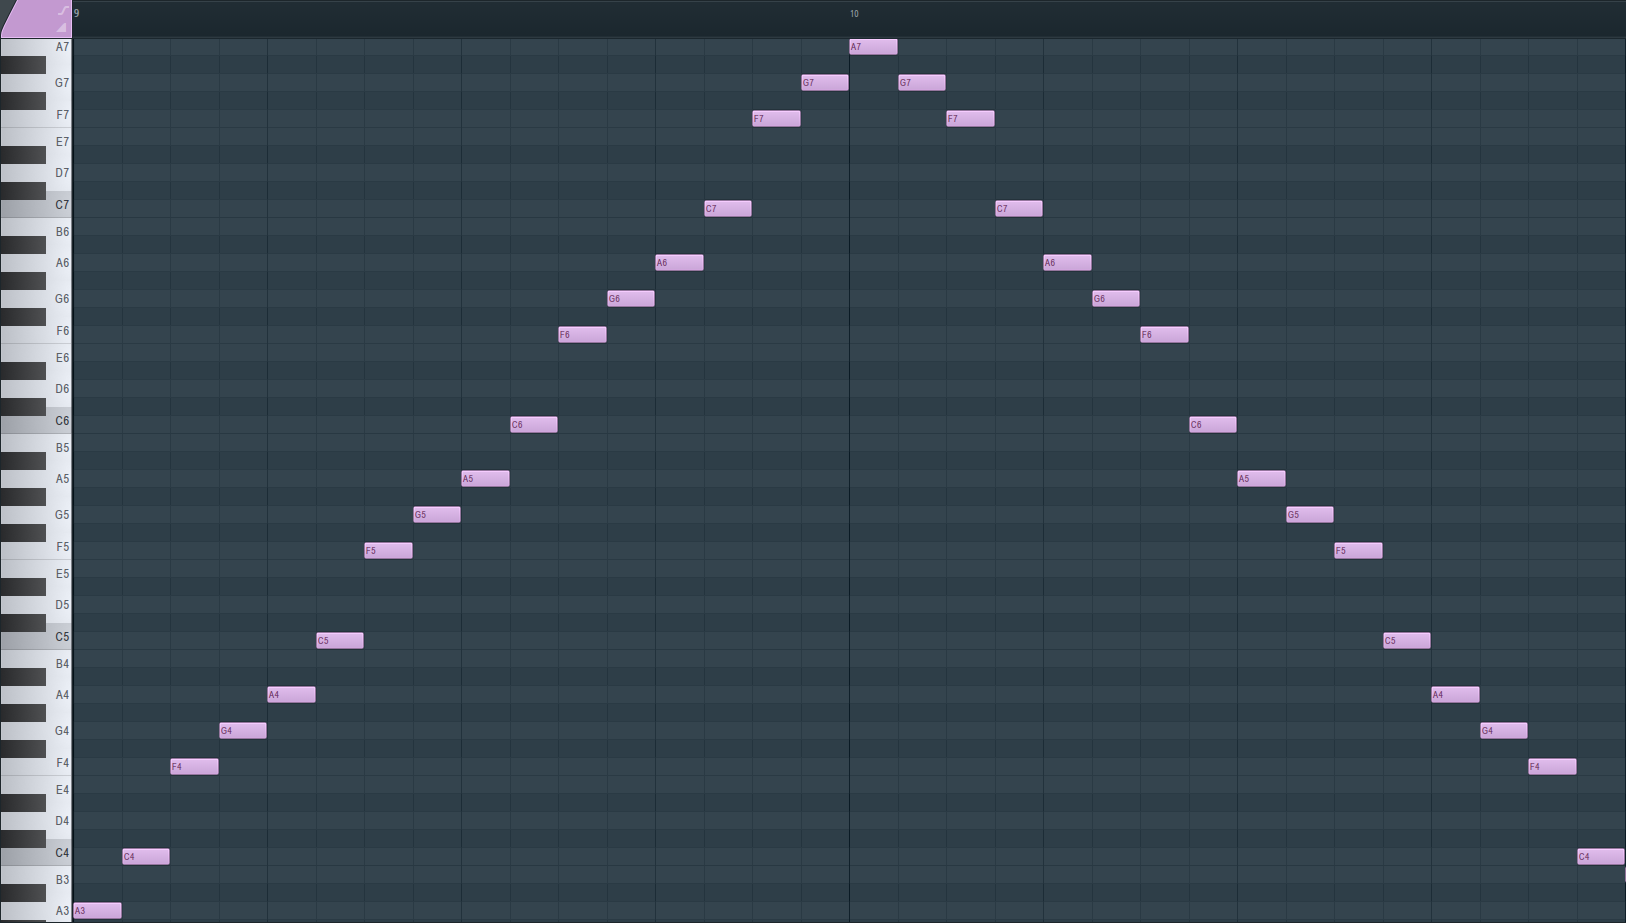
\includegraphics[width=.95\linewidth]{images/Noten_C.png}
	\caption{Notenabfolge C}
	\label{NotenabfolgeC}
\end{figure}

\begin{figure}[htbp] \centering
	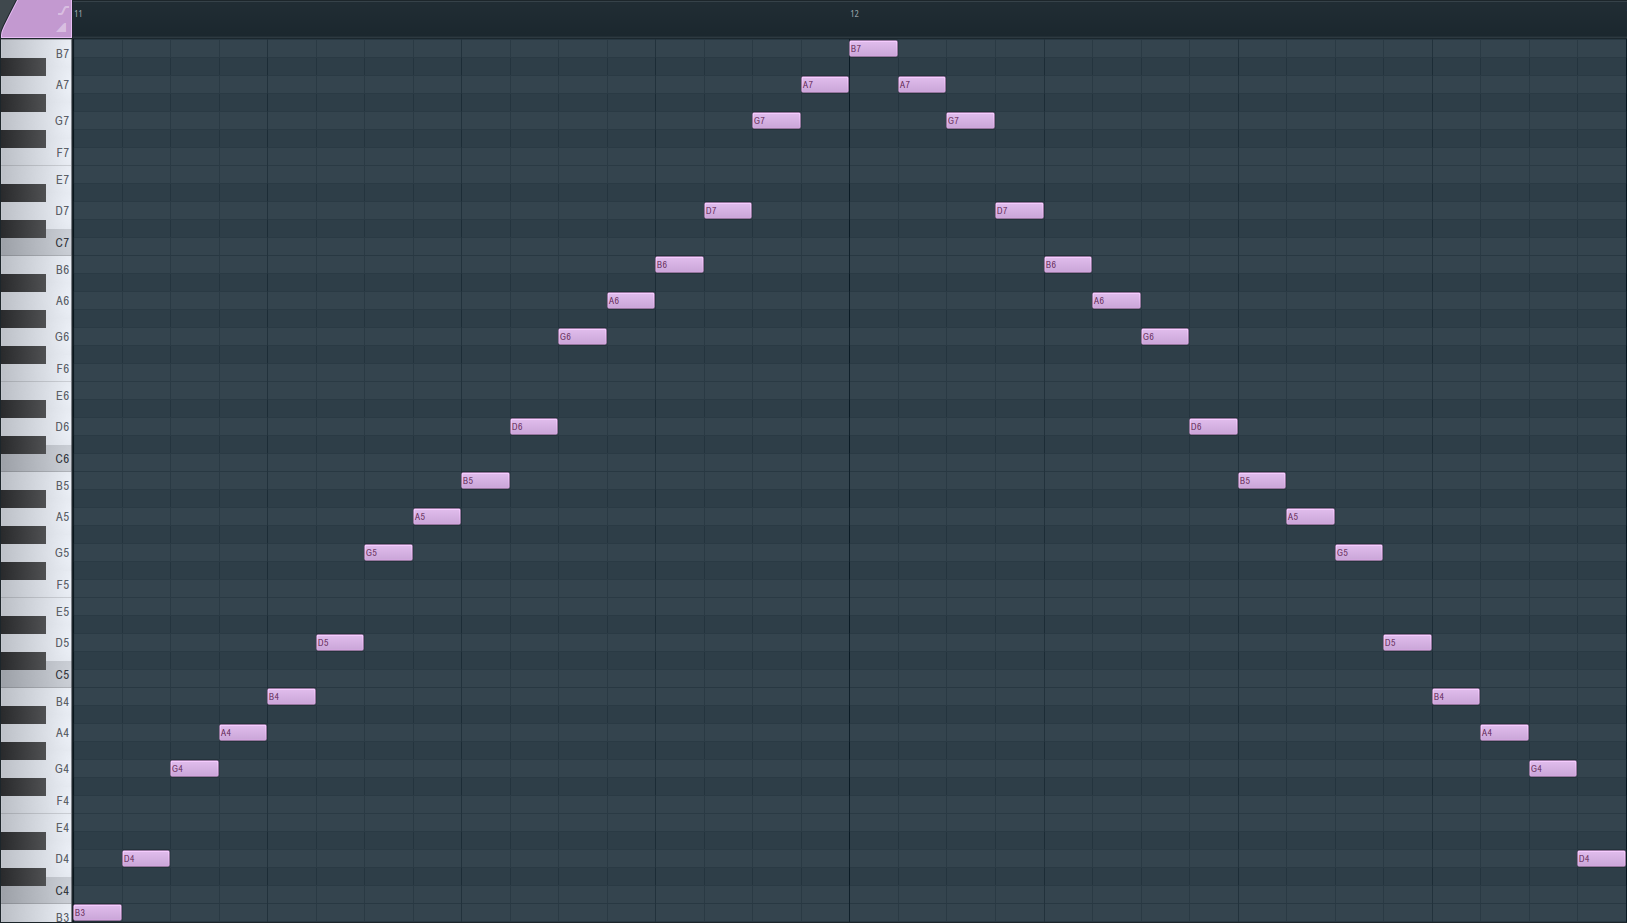
\includegraphics[width=.95\linewidth]{images/Noten_D.png}
	\caption{Notenabfolge D}
	\label{NotenabfolgeD}
\end{figure}

\begin{figure}[htbp] \centering
	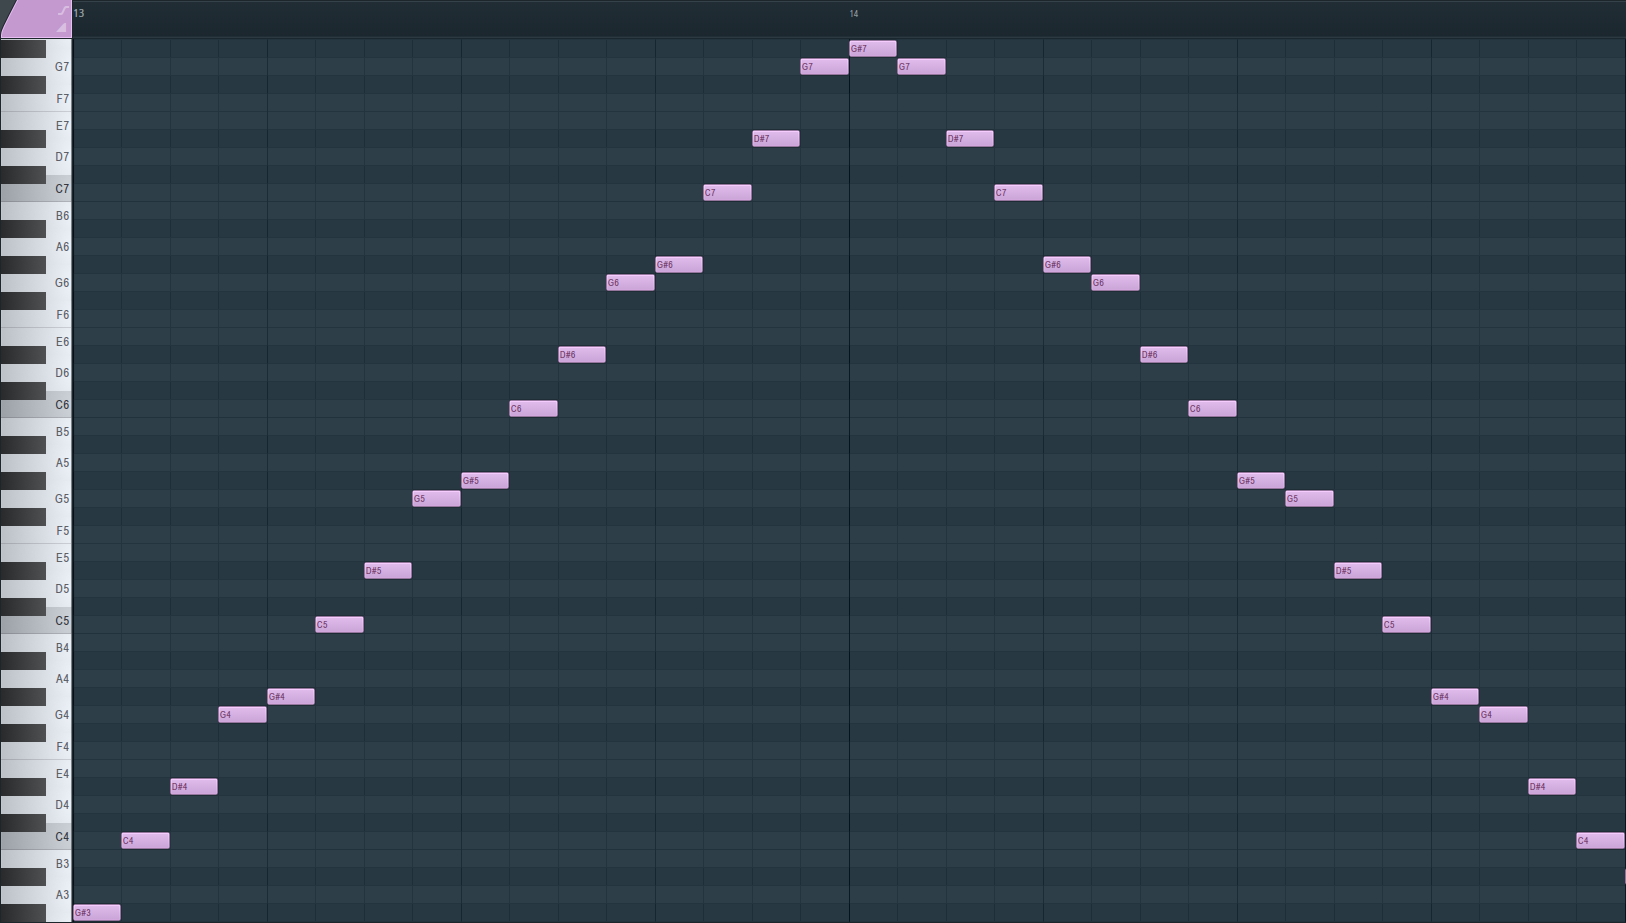
\includegraphics[width=.95\linewidth]{images/Noten_E.png}
	\caption{Notenabfolge E}
	\label{NotenabfolgeE}
\end{figure}

\begin{figure}[htbp] \centering
	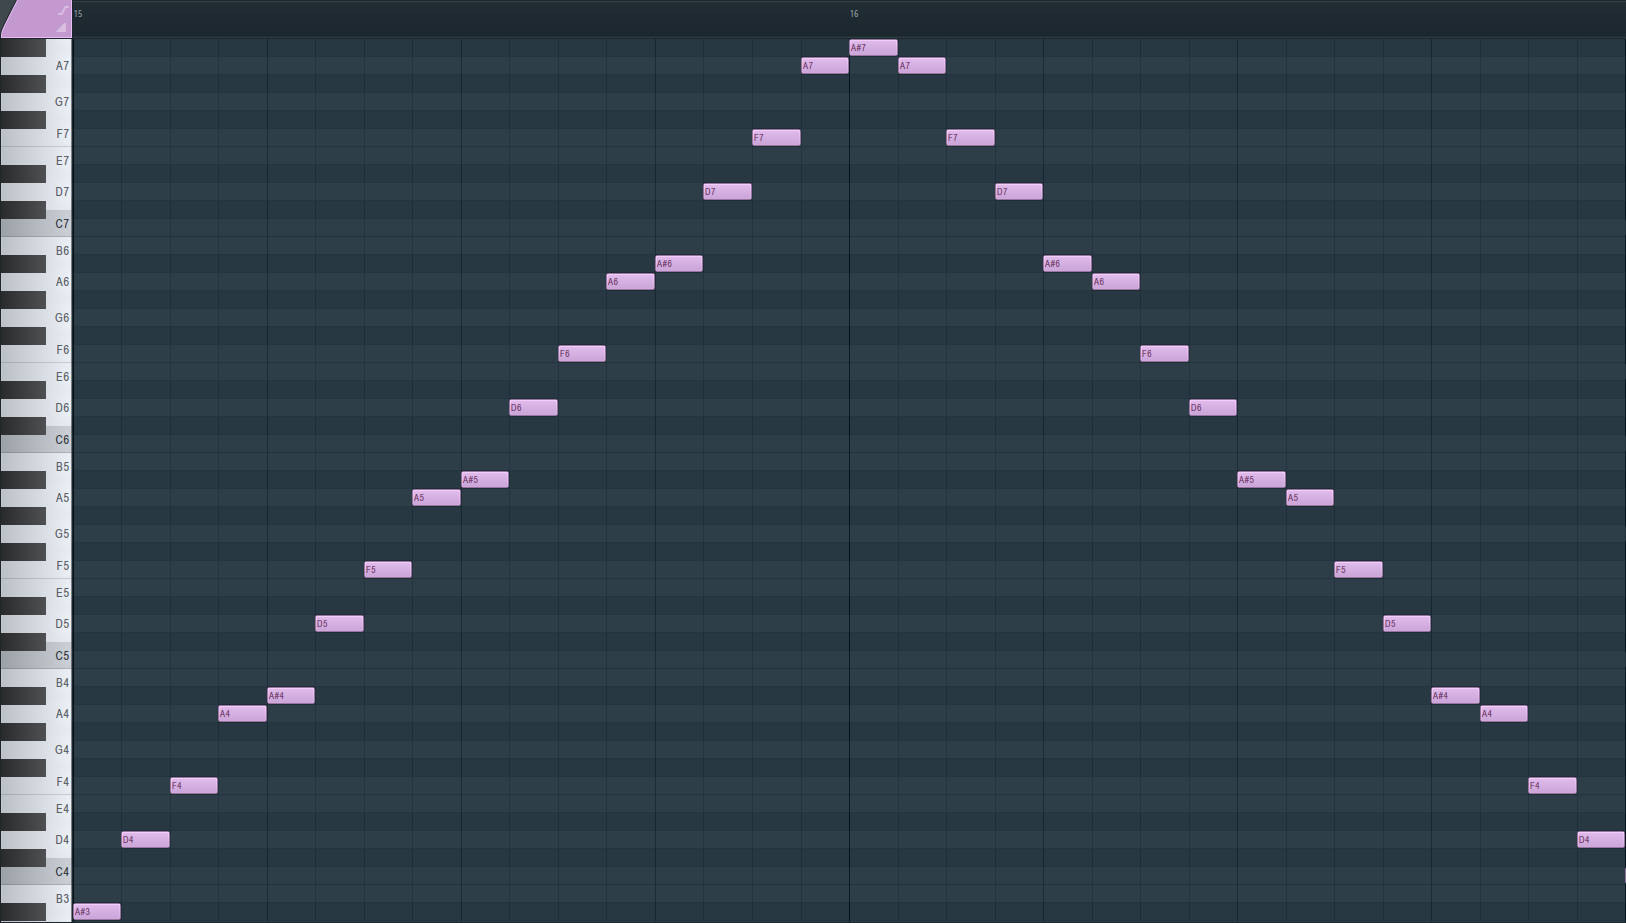
\includegraphics[width=.95\linewidth]{images/Noten_F.png}
	\caption{Notenabfolge F}
	\label{NotenabfolgeF}
\end{figure}


\begin{table}[htbp]
	\centering
	\begin{tabularx}{4.5cm}{|l|X|}
		\hline
		\$C0 & Ganze Note \\
		\hline
		\$80 & Ganze Triole \\
		\hline
		\$60 & Halbe Note \\
		\hline
		\$40 & Halbe Triole \\
		\hline
		\$30 & Viertelnote \\
		\hline
		\$20 & Viertel Triole \\
		\hline
		\$18 & Achtelnote \\
		\hline
		\$10 & Achtel Triole \\
		\hline
		\$0C & 16tel Note \\
		\hline
		\$09 & 16tel Triole \\
		\hline
		\$06 & 32tel Note \\
		\hline
		\$04 & 32tel Triole \\
		\hline
		\$03 & 64tel Note \\
		\hline
		\$02 & 64tel Triole \\
		\hline
	\end{tabularx}
	\caption{Längen in Hexwerte}
	\label{tickshex}
\end{table}



\end{document}
